%----------------------------------------------------------------------------------------
%	PACKAGES AND OTHER DOCUMENT CONFIGURATIONS
%----------------------------------------------------------------------------------------

\documentclass[fleqn,10pt]{Flavio}\usepackage[]{graphicx}\usepackage[]{color}
%% maxwidth is the original width if it is less than linewidth
%% otherwise use linewidth (to make sure the graphics do not exceed the margin)
\makeatletter
\def\maxwidth{ %
  \ifdim\Gin@nat@width>\linewidth
    \linewidth
  \else
    \Gin@nat@width
  \fi
}
\makeatother

\definecolor{fgcolor}{rgb}{0.345, 0.345, 0.345}
\newcommand{\hlnum}[1]{\textcolor[rgb]{0.686,0.059,0.569}{#1}}%
\newcommand{\hlstr}[1]{\textcolor[rgb]{0.192,0.494,0.8}{#1}}%
\newcommand{\hlcom}[1]{\textcolor[rgb]{0.678,0.584,0.686}{\textit{#1}}}%
\newcommand{\hlopt}[1]{\textcolor[rgb]{0,0,0}{#1}}%
\newcommand{\hlstd}[1]{\textcolor[rgb]{0.345,0.345,0.345}{#1}}%
\newcommand{\hlkwa}[1]{\textcolor[rgb]{0.161,0.373,0.58}{\textbf{#1}}}%
\newcommand{\hlkwb}[1]{\textcolor[rgb]{0.69,0.353,0.396}{#1}}%
\newcommand{\hlkwc}[1]{\textcolor[rgb]{0.333,0.667,0.333}{#1}}%
\newcommand{\hlkwd}[1]{\textcolor[rgb]{0.737,0.353,0.396}{\textbf{#1}}}%

\usepackage{framed}
\makeatletter
\newenvironment{kframe}{%
 \def\at@end@of@kframe{}%
 \ifinner\ifhmode%
  \def\at@end@of@kframe{\end{minipage}}%
  \begin{minipage}{\columnwidth}%
 \fi\fi%
 \def\FrameCommand##1{\hskip\@totalleftmargin \hskip-\fboxsep
 \colorbox{shadecolor}{##1}\hskip-\fboxsep
     % There is no \\@totalrightmargin, so:
     \hskip-\linewidth \hskip-\@totalleftmargin \hskip\columnwidth}%
 \MakeFramed {\advance\hsize-\width
   \@totalleftmargin\z@ \linewidth\hsize
   \@setminipage}}%
 {\par\unskip\endMakeFramed%
 \at@end@of@kframe}
\makeatother

\definecolor{shadecolor}{rgb}{.97, .97, .97}
\definecolor{messagecolor}{rgb}{0, 0, 0}
\definecolor{warningcolor}{rgb}{1, 0, 1}
\definecolor{errorcolor}{rgb}{1, 0, 0}
\newenvironment{knitrout}{}{} % an empty environment to be redefined in TeX

\usepackage{alltt} % Document font size and equations flushed left

%----------------------------------------------------------------------------------------
%	COLUMNS
%----------------------------------------------------------------------------------------

\setlength{\columnsep}{0.55cm} % Distance between the two columns of text
\setlength{\fboxrule}{0.75pt} % Width of the border around the abstract

%----------------------------------------------------------------------------------------
%	COLORS
%----------------------------------------------------------------------------------------

\definecolor{color1}{RGB}{0,0,90} % Color of the article title and sections
\definecolor{color2}{RGB}{0,20,20} % Color of the boxes behind the abstract and headings

%----------------------------------------------------------------------------------------
%	HYPERLINKS
%----------------------------------------------------------------------------------------

\usepackage{hyperref} % Required for hyperlinks
\hypersetup{hidelinks,colorlinks,breaklinks=true,urlcolor=color2,citecolor=color1,linkcolor=color1,bookmarksopen=false,pdftitle={Title},pdfauthor={Author}}

%----------------------------------------------------------------------------------------
%	ARTICLE INFORMATION
%----------------------------------------------------------------------------------------

\JournalInfo{Universidad Nacional Agraria la Molina} % Journal information
\Archive{Facultad de Agronom\'ia, 2015} % Additional notes (e.g. copyright, DOI, review/research article)

\PaperTitle{Evaluaci\'on de la eficiencia de uso de agua en quince genotipos de papa (\emph{Solanum tuberosum} L.) bajo condiciones de sequ\'ia controlada.} % Article title

\Authors{Lozano-Isla, Flavio\textsuperscript{*}; Farfan, Evelyn; Guti\'errez, Raymundo; Blas, Ra\'ul\textsuperscript{1}} % Authors

\affiliation{\textsuperscript{1}\textit{Departamento de Fitot\'ecnia, Universidad Nacional Agraria la Molina, Lima, Per\'u}} % Author affiliation
\affiliation{*\textbf{Correspondencia}: F.lozano@outlook.com} % Corresponding author

\Keywords{ Papa ---  Eficiencia de uso de agua ---  \'Indice de cosecha ---  Tolerancia a la sequ\'ia} % Keywords - if you don't want any simply remove all the text between the curly brackets
\newcommand{\keywordname}{Palabras Claves} % Defines the keywords heading name

%----------------------------------------------------------------------------------------
%	ABSTRACT
%----------------------------------------------------------------------------------------

\addto{\captionsenglish}{\renewcommand{\abstractname}{Resumen}}
\Abstract{La papa (\emph{Solanum tuberosum} L.) es un cultivo sensible a la sequ\'ia debido a que posee un sistema radicular poco profundo y requiere disponibilidad constante de agua en el suelo para asegurar su m\'aximo rendimiento y calidad en el tub\'erculo. La eficiencia de uso de agua (EUA) se define como la producci\'on por unidad de agua consumida, esta variable es considerada importante para determinar el rendimiento bajo condiciones limitadas de agua. Si logramos entender la relaci\'on entre EUA y el rendimiento bajo condiciones de estr\'es puede ayudarnos a encontrar estrategias que nos ayuden a minimizar la perdida de rendimiento debido a la disponibilidad de agua y asegurar una alta producci\'on. Se llev\'o acabo un experimento en invernadero con condiciones controladas , para caracterizar la respuesta y entender la relaci\'on entre la EUA, el rendimiento y la tolerancia en 15 genotipos de papa de la poblaci\'on avanzada de mejoramiento del Centro Internacional de la Papa (CIP). El experimento fue llevado acabo baja el dise\~no experimental de parcelas divididas teniendo como factor principal dos tipos de riego, sequ\'ia regulada y riego normal y como factor secundario los quince genotipos. A trav\'es del experimento se evaluaron variables morfol\'ogicas y fisiol\'ogicas tales como contenido relativo de clorofila (SPAD), \'area foliar (AF) , transpiraci\'on y par\'ametros de rendimiento tales como el peso de la biomasa, \'indice de cosecha (IC) e \'indice de tolerancia a la reducci\'on de agua (TRA). Los resultados de la investigaci\'on muestran diferencias significativas entre tratamientos, las plantas sometidas a limitaciones de agua muestran un rendimiento menor, existiendo una reducci\'on en la biomasa y el \'area foliar. Existe una correlaci\'on alta entra la EUA y el IC ($r = 0.98$), indicando que este \'ultimo puede ser una herramienta \'util para la selecci\'on prematura de genotipos con buen rendimiento y tolerante al estr\'es por sequ\'ia. Los genotipos CIP398190.89, CIP397077.16, CIP392797.22, CIP398208.620 mostraron una mayor eficiencia en el uso de agua bajo condiciones de sequ\'ia sin que esto produzca una reducci\'on dr\'astica en su rendimiento.}


%----------------------------------------------------------------------------------------
\IfFileExists{upquote.sty}{\usepackage{upquote}}{}
\begin{document}

\flushbottom % Makes all text pages the same height
\maketitle % Print the title and abstract box
%\tableofcontents % Print the contents section
%\thispagestyle{empty} % Removes page numbering from the first page

%----------------------------------------------------------------------------------------
%	ARTICLE CONTENTS
%----------------------------------------------------------------------------------------

\section*{Introducci\'on} % The \section*{} command stops section numbering
\addcontentsline{toc}{section}{Introducc\'ion} % Adds this section to the table of contents

La papa es el tercer cultivo m\'as importante despu\'es del trigo y el arroz a nivel mundial. Sin embargo, poco se conoce de la importancia que tiene este tub\'erculo para la salud y la alimentaci\'on humana. El consumo de 100 g de papas al d\'ia,  puede cubrir el requerimiento de hasta el 50 \% de las necesidades de vitamina C para el ser humano \citep{INIAP18/06/14}. . Adem\'as, es la base de la alimentaci\'on de la zona andina y es producido por 600 mil peque\~nas unidades agrarias. La siembra promedio es de 274,411 hect\'areas en 19 regiones del Per\'u. Puede desarrollarse desde el nivel del mar hasta los 4,200 m.s.n.m.; pero mayormente prospera en climas semitemplados. El rendimiento promedio nacional es de 13.3 t/ha. En costa el promedio alcanza a 25 t/ha. Esto tambi\'en depende de la variedad de papa, niveles de fertilizaci\'on y condiciones de riego. El Per\'u es el pa\'is con mayor diversidad de papas cultivadas en el mundo, al contar con 8 especies nativas domesticadas y 2600 de las m\'as de 4000 variedades que existen en Latinoam\'erica. Adem\'as, nuestro pa\'is posee 91 de las 200 especies que crecen en forma silvestre en casi todo nuestro continente \citep{MINAG18/06/14}. 

La falta de agua o d\'eficit h\'idrico se representa como la tensi\'on o estr\'es que actuar\'ia sobre las plantas, y toda tensi\'on produce dos tipos de respuesta en los organismos: respuestas que tienden a evitar o prevenir la tensi\'on (mecanismos evitadores) y mecanismos o adaptaciones que permiten soportar o resistir el estr\'es (mecanismos de tolerancia). Mientras todas las estrategias de tolerancia conllevan una limitaci\'on mayor o menor del crecimiento, solo la estrategia de ahorro de agua conlleva un crecimiento limitado en el caso de la evitaci\'on del estr\'es. Las especies que derrochan agua son en general m\'as productivas y tienen mecanismos que les permiten una eficaz extracci\'on del agua del sustrato y una elevada conductividad hidr\'aulica interna para abastecer con rapidez toda la parte a\'erea de la planta. Esto les confiere una gran competitividad, pero no es siempre una estrategia viable en medios secos, particularmente cuando la carencia de agua es cr\'onica. En estas condiciones predominan las especies tolerantes del estr\'es h\'idrico \citep{Valladares2004}. 


Para rendimientos altos, el requerimiento de agua del cultivo para  plantaciones de 120 a 150 d\'ias es de 500 a 700 mm dependiendo del clima. La relaci\'on entre la m\'axima evapotranspiraci\'on (ETm) y la evapotranspiraci\'on de referencia (ETo) es dada por el coeficiente del cultivo (Kc). Durante su etapa inicial el Kc del cultivo de papa es 0.4 - 0.5 (20 a 30 d\'ias), en la etapa de desarrollo es 0.7 - 0.8 (30 a 40 d\'ias) en la media estaci\'on de 1.05 a 1.2 (30 a 60 d\'ias), en la etapa tard\'ia de 0.85 - 0.95 (20 a 35 d\'ias) y en la madurez 0.7 - 0.75. En condiciones de secano se ha observado que una precipitaci\'on de 600 a 800 mm distribuidos regularmente durante el periodo vegetativo del cultivo de la papa es adecuada para obtener un buen rendimiento \citep{Barrantes1993}. El cultivo de papa es particularmente sensible a la sequ\'ia \citep{Yuan2003} en consecuencia requiere un adecuado riego para mantener el rendimiento y la calidad de los tub\'erculos \citep{Porter1999,Fabeiro2001}. Para optimizar el rendimiento total del agua disponible en el suelo no debe ser agotado por m\'as de 30 a 50 \%. El agotamiento de la cantidad total de agua disponible en el suelo durante el per\'iodo de crecimiento de m\'as del 50 \% da como resultados rendimientos m\'as bajos. El d\'eficit de agua durante el per\'iodo de estolonizaci\'on e iniciaci\'on del tub\'erculo y la formaci\'on de rendimiento tienen el mayor efecto adverso en el rendimiento, mientras que la maduraci\'on  y la etapa vegetativa temprana son per\'iodos menos sensibles. Un buen rendimiento del cultivo de papa de 120 d\'ias en climas templados y subtropical es de 25 a 35 t/ha de tub\'erculos frescos y en climas tropicales los rendimientos son de 15 a 25 t/ha. La eficiencia de utilizaci\'on del agua para la producci\'on cosechada de tub\'erculos que contienen de 70 a 75 por ciento de humedad es de 4 a 7 $kg/m^3$ \citep{FAO18/06/14}.


El presente trabajo tiene como objetivo evaluar distintos par\'ametros fisiol\'ogicos y morfol\'ogicos para relacionarlo con la eficiencia de uso de agua y el rendimiento del cultivo y seleccionar los genotipos de papa que presenten tolerancia al estr\'es h\'idrico por sequ\'ia con rendimientos aceptables. Para evaluar la eficiencia de uso de agua en los 15 genotipos de estudio, se utiliz\'o la metodolog\'ia del lis\'imetro, que permite calcular la transpiraci\'on o consumo de agua neta de las plantas. Durante el desarrollo del experimento se realizaron evaluaciones morfol\'ogicas y fisiol\'ogicas para observar los mecanismos que utilizan las plantas de papa para tolerar el estr\'es por sequ\'ia. Los datos extra\'idos se correlacionaron con los rendimientos para determinar cu\'ales de las variables presentan mayor respuesta a la sequ\'ia.


%------------------------------------------------

\section{Materiales y M\'etodos}

\subsection{Material biol\'ogico}

Se utilizaron quince (15) genotipos de papa provenientes de poblaciones de mejoramiento del Centro Internacional de la Papa. Los cuales fueron evaluados y seleccionados por sus buenas caracter\'isticas agron\'omicas y bromatol\'ogicas. Dentro del grupo de genotipos empleados se usaron 2 variedades de papa (UNICA y Achirana) que fueron evaluados bajo condiciones de sequ\'ia en experimentos anteriores por lo que se tiene conocimiento de su tolerancia al estr\'es por sequ\'ia. Los genotipos presentan distintas caracter\'isticas en su precocidad y madurez fisiol\'ogica (Tabla \ref{tab:genotypes2}).

\begin{table*}[ht]\centering
\caption{Informaci\'on agron\'omica de los 15 genotipos de papa evaluados}
\centering
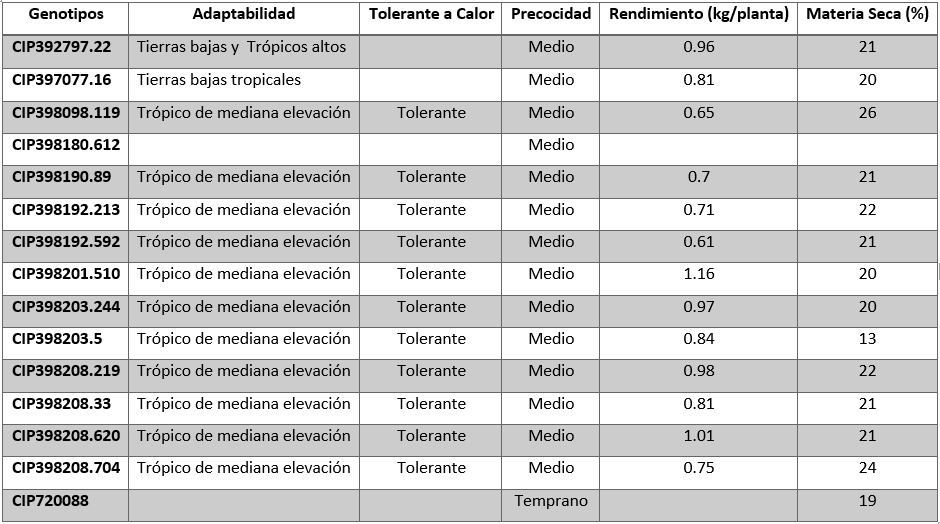
\includegraphics[width=\linewidth]{genotypes}
\label{tab:genotypes2}
\end{table*}

\subsection{Localizaci\'on y condiciones ambientales}
	
El presente trabajo de investigaci\'on se desarroll\'o en el invernadero del Centro Internacional de la papa. El experimento se llev\'o  acabo en la estaci\'on  de invierno  (Mayo a Agosto de 2013). Las temperaturas promedio m\'axima y m\'inima  del invernadero fueron de 24 y 15 $^{\circ}$C respectivamente. La humedad relativa promedio fue de 80 \%. No hubo uso de luz artificial.
		
\subsection{Establecimiento de experimento}

La desinfecci\'on de los materiales usados en la siembra, se realiz\'o con 30 g de hipoclorito de calcio en 120 litros de agua. Se sumergieron los materiales para su desinfecci\'on (macetas, tutores de bamb\'u y mallas pl\'asticas). Luego se procedi\'o a enjugar y ponerlos a secar para su uso posterior. Se utiliz\'o una mezcla de sustrato SOGEMIX SM-2 (75 \% Musgo de turba, perlita, vermiculita, y la piedra caliza) mezclada con tierra de chacra proveniente de la estaci\'on experimental de Huancayo. La desinfecci\'on del sustrato se realiz\'o con vapor de agua (100 $^{\circ}$C) por 8 horas y luego se dej\'o a la intemperie para su enfriado, luego de 48 horas se procedi\'o a realizar un muestreo del sustrato para su an\'alisis. Cada maceta fue tarada y se coloc\'o 2 Kg de sustrato con una malla pl\'astica en la base para evitar la p\'erdida de sustrato. La fertilizaci\'on se fraccion\'o en dos, a la siembra y a los 40 d\'ias despu\'es de la siembra (DDS) en una dosis 170 - 60 - 270 de nitrato de amonio, superfosfato triple y sulfato de potasio respectivamente \citep{CIP23/06/14}.Los tub\'erculos fueron propagados en la estaci\'on experimental de Huancayo. Los tub\'erculos aun no brotados, fueron sometidos aun un tratamiento qu\'imico con RINDITE en una dosis de 200 ml en una c\'amara de 1 $m^3$ bien sellada por 72 horas, para romper la dormancia y luego se ponen los tub\'erculos en c\'amara caliente para favorecer el brotamiento de las yemas. Una vez que las semillas (tub\'erculo) estuvieron bien brotados se llevaron a c\'amara de luz difusa  para suberificar las yemas y proceder a sembrarlas.

\subsection{Tratamiento de riego}

Las plantas se regaron interdiariamente hasta el inicio del tratamiento. A los 30 DDS las macetas se saturaron con agua y se dejaron drenar durante la noche para eliminar el exceso de agua, las macetas fueron selladas con bolsas de polietileno para evitar la p\'erdida de agua por evaporaci\'on de la superficie del suelo, se realiz\'o el peso interdiario de las macetas hasta los 45 DDS para calcular los par\'ametros iniciales para la aplicaci\'on de los tratamientos (Fig. \ref{fig:pots}). El tratamiento de sequ\'ia regulada se inici\'o a los 45 DDS, con la metodolog\'ia de lis\'imetro. Se pesaron las macetas cada 2 d\'ias por las tardes (entre 13:00 y 15:00 horas) seg\'un la metodolog\'ia descrita en \citet{Bhatnagar-Mathur2007}. Con el fin de exponer a una sequ\'ia progresiva a las plantas en sequ\'ia controlada, se les redujo 150 ml de agua en cada riego, y las plantas con tratamiento de riego normal se le prove\'ia de agua de acuerdo a su demanda de transpiraci\'on, el c\'alculo se realiz\'o en base a la diferencia de pesos. La disminuci\'on del agua en el sustrato se puede graficar en base a los c\'alculos de la fracci\'on transpirable del suelo (Fig. \ref{fig:FTS}). Siendo el peso inicial de la maceta despu\'es de saturaci\'on la base para reponer el agua (capacidad de campo).

\begin{figure}[ht]\centering
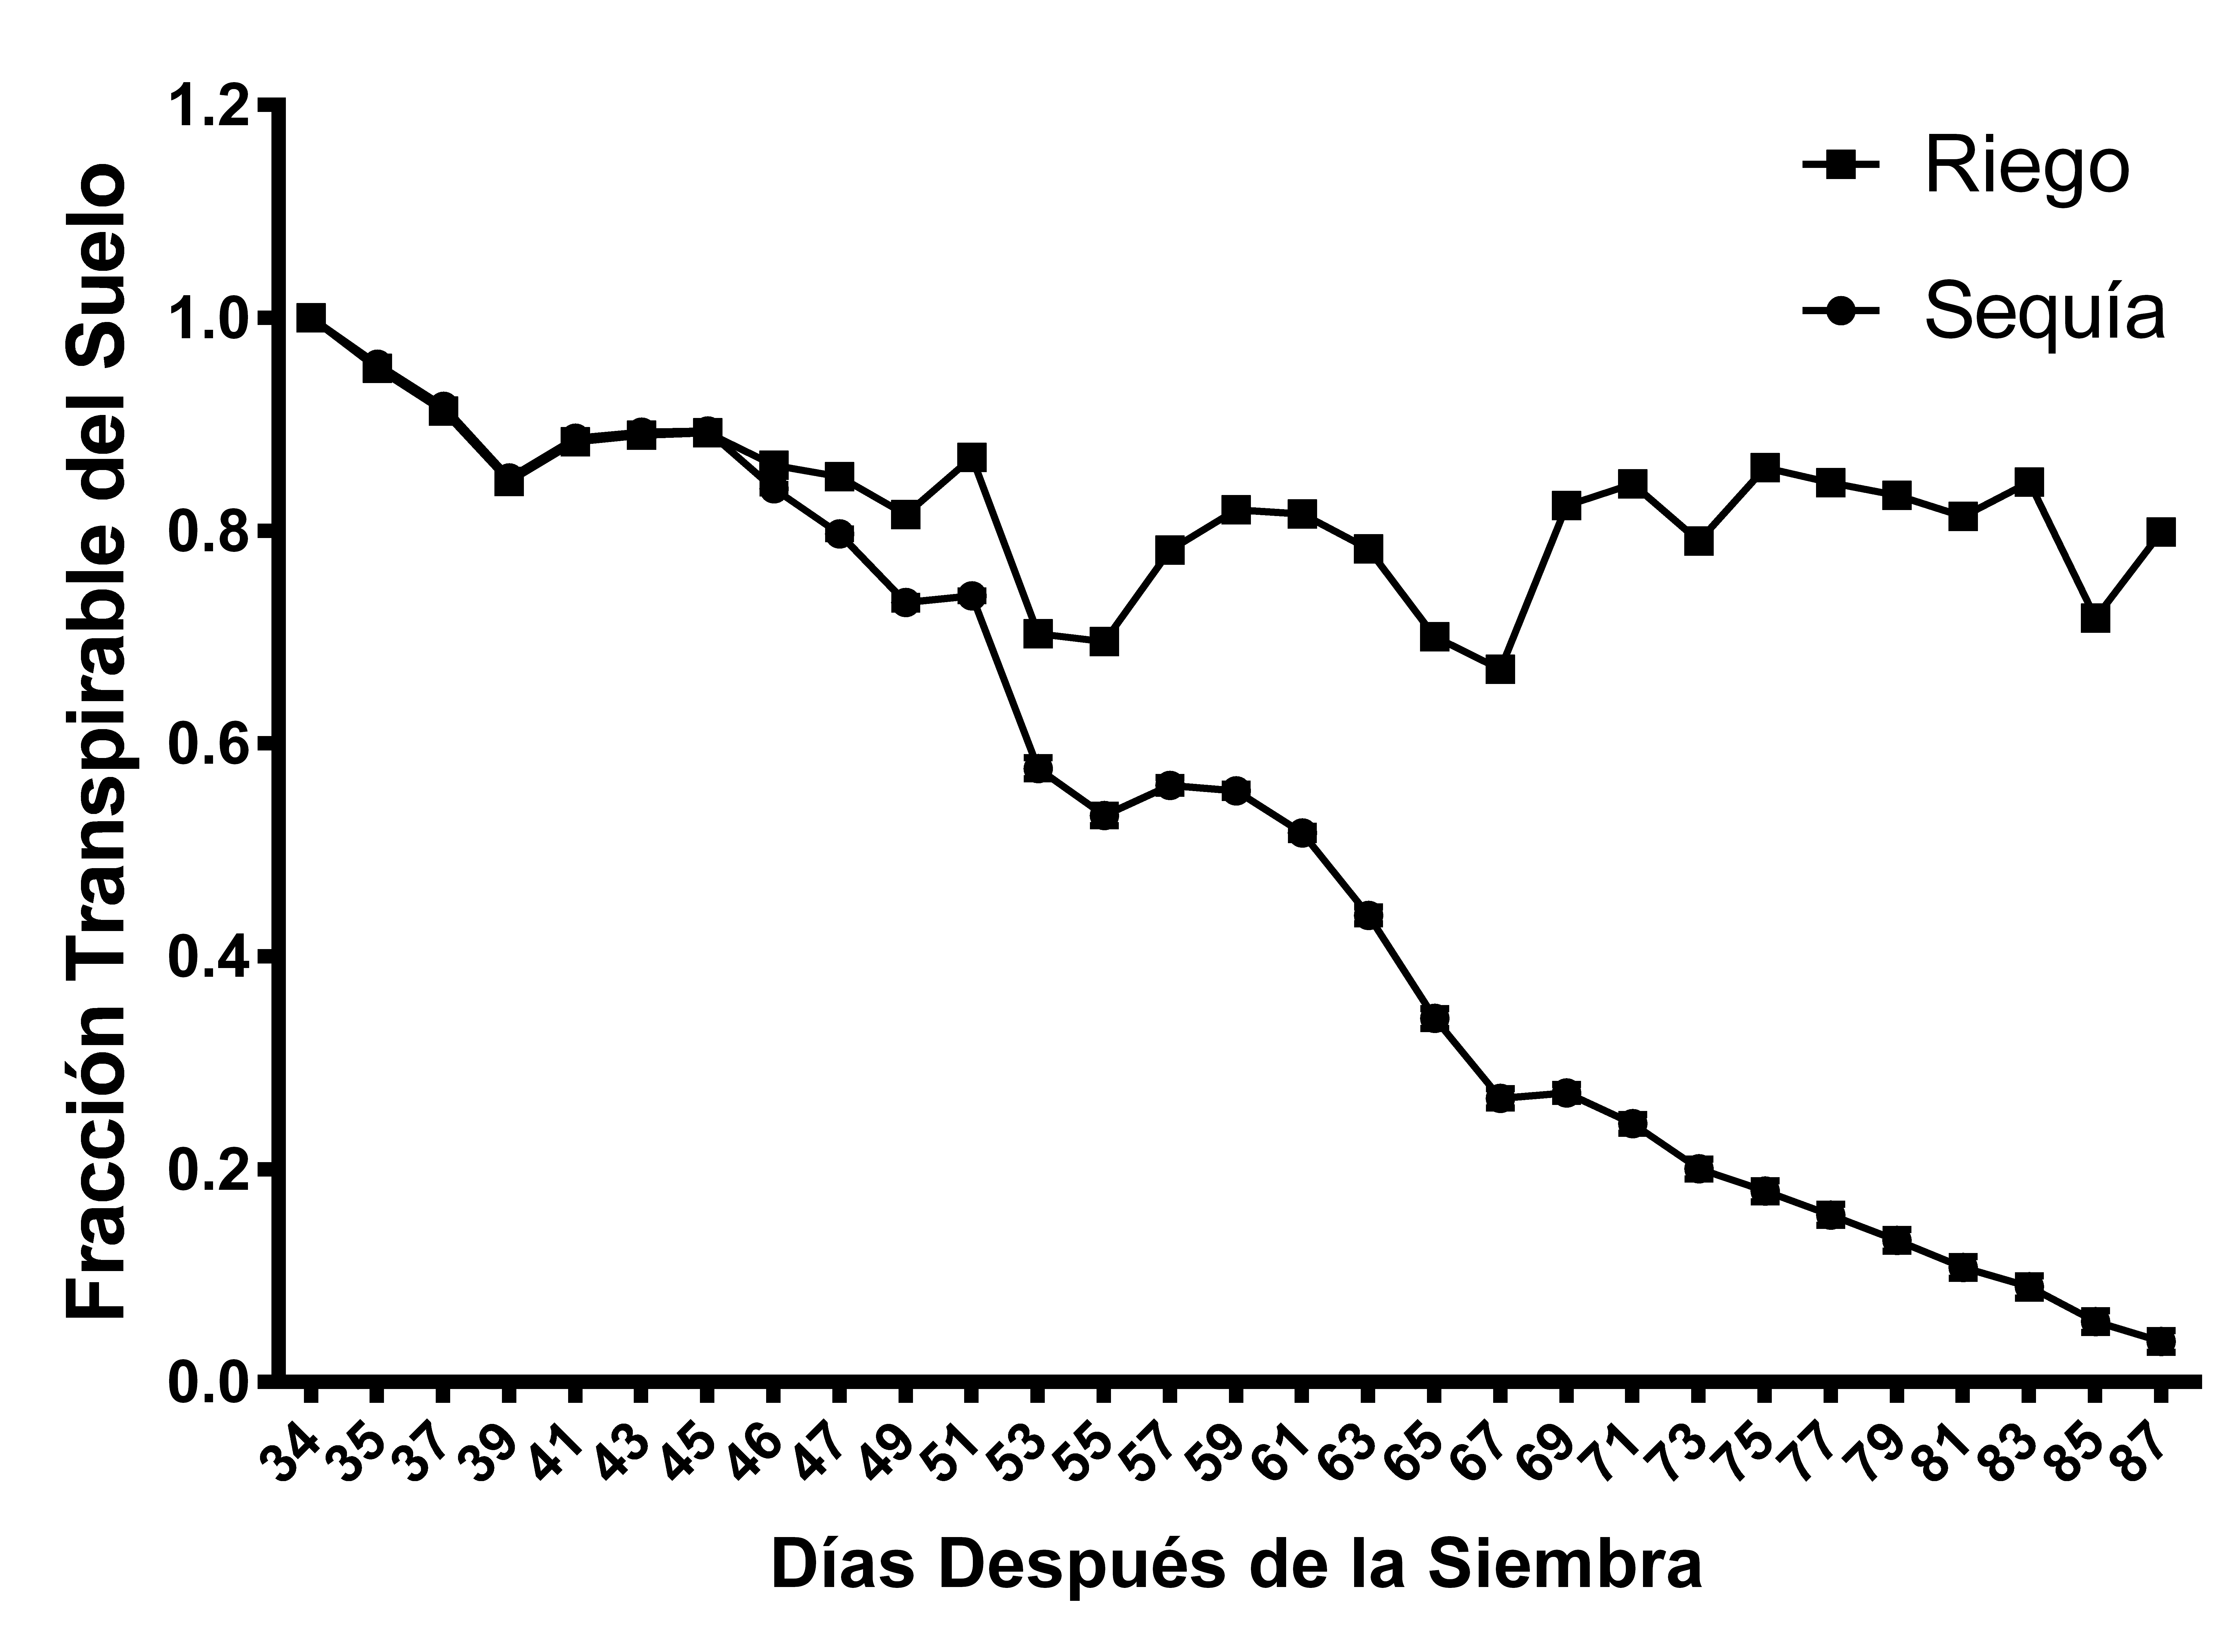
\includegraphics[width=\linewidth]{FTS}
\caption{Fracci\'on transpirable del suelo durante el tratamiento de sequ\'ia controlada}
\label{fig:FTS}
\end{figure}

\begin{figure}[ht]\centering
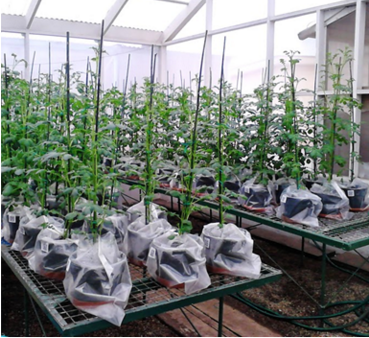
\includegraphics[width=\linewidth]{pots}
\caption{Sellado de macetas para evitar p\'erdidas de agua  por evaporaci\'on}
\label{fig:pots}
\end{figure}

\subsection{Variables evaluadas}

\paragraph{Componentes del rendimiento} Se separ\'o la planta en cuatro componentes (ra\'iz, tallo, hojas y tub\'erculos) a la cosecha se procedi\'o a pesar la biomasa fresca (g), luego se puso a la estufa a 80 $^{\circ}$C por 3 d\'ias, y se realiz\'o los pesos secos (g) por cada componente.

\begin{enumerate}[a),noitemsep]
  \item {\bf Biomasa seca (g)} Se determin\'o como las suma de los cuatro componentes: ra\'iz, tallo, hojas y tub\'erculos. 
  \item {\bf \'indice de cosecha} Se calcul\'o en base al peso seco de los componentes. Es la relaci\'on del peso seco del tub\'erculo en relaci\'on al peso de la biomasa
\end{enumerate}

\paragraph{Potencial osm\'otico} Para esta medici\'on se seleccion\'o un fol\'iolo de la tercera hoja extendida desde el \'apice de la planta y luego utilizando un sacabocado de 5 mm de di\'ametro, se extrajeron dos discos de dicho fol\'iolo. Estos se colocaron en viales criog\'enicos (NALGENE) de 1.0 ml, e inmediatamente se guardaron en nitr\'ogeno l\'iquido. Se realizaron las lecturas del potencial osm\'otico utilizando un microvolt\'imetro HR-33T  (Wescor Inc., Logan, UT, USA) y c\'amaras psicrom\'etricas C52 (Wescor Inc., Logan, UT, USA).Las muestras permanecieron durante 30 minutos  en las c\'amaras psicrometricas hasta alcanzar el equilibrio del punto de roc\'io; y en ese instante se procedi\'o a la lectura del dato.

\paragraph{Transpiraci\'on Total} Transpiraci\'on de las plantas se calcul\'o bajo la metodolog\'ia del lis\'imetro y se determina como la diferencia de pesos de las macetas, m\'as el agua a\~nadida en la evaluaci\'on anterior. La diferencia entre el peso inicial y final de la maceta permite estimar la transpiraci\'on total de agua del suelo disponible en cada maceta. Esta informaci\'on es utilizada para determinar la fracci\'on transpirable del suelo y calcular la cantidad de agua a reponerse en cada maceta. El c\'alculo de la fracci\'on transpirable del suelo (FTS) fue calculada usando la siguiente formula:

$$ FTS = \left(\frac{1 - PIM - PDM}{PIM - PFM}\right) $$

Donde:

\begin{itemize}[noitemsep]
  \item FTS: Fracci\'on Transpirable del Suelo 
  \item PIM (g): Peso Inicial de la Maceta 
  \item PDM (g): Peso Diario de la Maceta 
  \item PFM (g): Peso Final de la Maceta 
\end{itemize}


\paragraph{\'Area foliar} El \'area foliar representa la superficie total de la hoja en $cm^2$. Se realiz\'o a los 90 DDS, al t\'ermino del experimento, la evaluaci\'on de realiz\'o en cada unidad experimental. Las hojas cosechadas se colocaron sobre una superficie y se tom\'o una foto perpendicular a la superficie captando todas las hojas, luego se procedi\'o a su an\'alisis en el Software SisCop v1.0 (Embrapa Instrumentacao Agropecuaria, 2003)

\paragraph{Eficiencia de uso de agua} El uso eficiente de agua est\'a definido como proporci\'on de biomasa acumulada, expresada como di\'oxido de carbono asimilado por el cultivo por cantidad de agua consumida, expresada como transpiraci\'on, evapotranspiraci\'on o total de agua ingresada al sistema \citep{Sinclair1984}. Para el caso de este estudio se utilizara la eficiencia de uso de agua en tub\'erculos (EUAtuberculos) y biomasa total (EUAbiomasa).

$$ EUA = \left(\frac{PS_{biomasa}}{TT}\right) $$

Donde:

\begin{itemize}[noitemsep]
\item $PS_{biomasa}$ (g): Peso Seco de Tub\'erculo y/o biomasa total 
\item TT (ml): Transpiraci\'on Total
\end{itemize}

\paragraph{Contenido relativo de clorofila} Es el contenido relativo de pigmentos fotosint\'eticos medido con un equipo de desarrollo anal\'itico de suelos y plantas (soil plant analytical development, SPAD). El an\'alisis de las clorofilas da a conocer el estado de desarrollo de la planta y permite la determinaci\'on del estado fisiol\'ogico de la planta, con lo cual se puede detectar posibles estreses \citep{Ferri2004}.Para realizar esta medici\'on, se us\'o el clorofil\'ometro (Konica Minolta Sensing, Inc., Osaka, Japan). Se seleccionaron tres  foliolos un impar y los dos pares cercanos a este, de la tercera hoja extendida desde la parte apical de la planta. En los cuales se realiz\'o tres lecturas o muestreos, por cada fol\'iolo y se promediaron  dichas lecturas por cada unidad experimental. Las unidades de medici\'on son caracter\'istica del equipo, las cuales figuran como unidades SPAD (por sus siglas en ingl\'es: Soil Plant Analizer Device) las cuales representan o equivalen al contenido relativo de clorofila en la hoja de la planta.

\paragraph{\'Indice de tolerancia a la reducci\'on de agua} El \'indice de sequ\'ia, Tolerancia a la Reducci\'on de Agua (TRA), es usado para caracterizar la respuesta de cada genotipo sometido a condiciones de sequ\'ia. Es calculado como el peso seco tub\'erculo en condiciones de sequ\'ia en relaci\'on al peso seco del tub\'erculo en condiciones de riego \citep{Deblonde2001}. El \'indice de tolerancia a la reducci\'on de agua depende no solo del rendimiento bajo sequ\'ia y riego, sino tambi\'en de la intensidad del estr\'es. Este valor depende altamente de las condiciones ambientales. Valores menores a la unidad son considerados tolerantes a la sequ\'ia, ya que la reducci\'on en condiciones de sequ\'ia es m\'as peque\~na que el rendimiento promedio de todo los genotipos evaluados \cite{Cabello2013}. El TRA se calcula mediante la expresi\'on:

$$ TRA =   \frac { 1 - (\frac{Y_s}{Y_p}) } { 1 - (\frac{Y_{ms}}{Y_{mp}}) } $$


Donde:

\begin{itemize}[noitemsep]
  \item TRA   : Tolerancia a la reducci\'on del agua. 
  \item $Y_s$ : Rendimiento bajo sequ\'ia. 
  \item $Y_p$ : Rendimiento bajo condiciones de riego. 
  \item $Y_{ms}$ : Rendimiento promedio de los genotipos bajo sequ\'ia.
  \item $Y_{mp}$ : Rendimiento promedio de los genotipos bajo condiciones de riego. 
\end{itemize}


\subsection{Dise\~no y an\'alisis estad\'istico}

El dise\~no experimental utilizado fue de Parcelas Divididas, lo cual es adecuado para la caracter\'isticas de la evaluaci\'on \citep{Montgomery1999}. La unidad experimental fue de una planta y/o maceta. Los factores por analizar fueron dos: los genotipos de papa y los tipos de riego. El factor genotipos const\'o de 13 clones avanzado y 2 variedades comerciales de papa  (UNICA y Achirana) . El factor de tipo de riego tuvo dos tratamientos: riego normal y sequ\'ia controlada. Las unidades experimentales fueron cinco por tratamiento las que fueron distribuidas al azar. Los datos fueron procesados y analizados en el software Estad\'istico R v.3.0.3 (The R Foundation for Statistical Computing). Los datos previos a su an\'alisis fueron sometidos a detecci\'on de ``valores at\'ipicos' usando el paquete ``car'', para los an\'alisis de variancia (ANVA) y correlaci\'on de Pearson en el paquete ``Agricolae''. El an\'alisis de componentes principales con ``FactoMineR''. Los An\'alisis de regresi\'on lineal y figuras se realiz\'o con el software estad\'istico GraphPad Prism 6 (GraphPad Software, Inc.). 


%------------------------------------------------

\section{Resultados}

\subsection{Clones con tolerancia al estr\'es por sequ\'ia en base al rendimiento } 

Los resultados muestran que no existe interacci\'on entre los tratamientos con los genotipos. Pero si existe diferencias significativas entre los tratamientos, siendo el tratamiento de riego controlado el que present\'o mayor rendimiento (40.61 g/planta) con respecto a las plantas en sequ\'ia regulada (23.87 g/planta) (Fig \ref{fig:tpic}).Los genotipos que presentaron mayor rendimiento fueron CIP398208.620 con 53.15 g; CIP398098.119 con 50.18 g y el CIP398208.219 con 43.83 g. Mientras que los genotipos contrastantes fueron CIP720088 con 19.35 gr; CIP398201.510 con 18.68 g  y el CIP398203.244 con 8.59 g (Fig \ref{fig:yield}).

\begin{figure}[ht]\centering
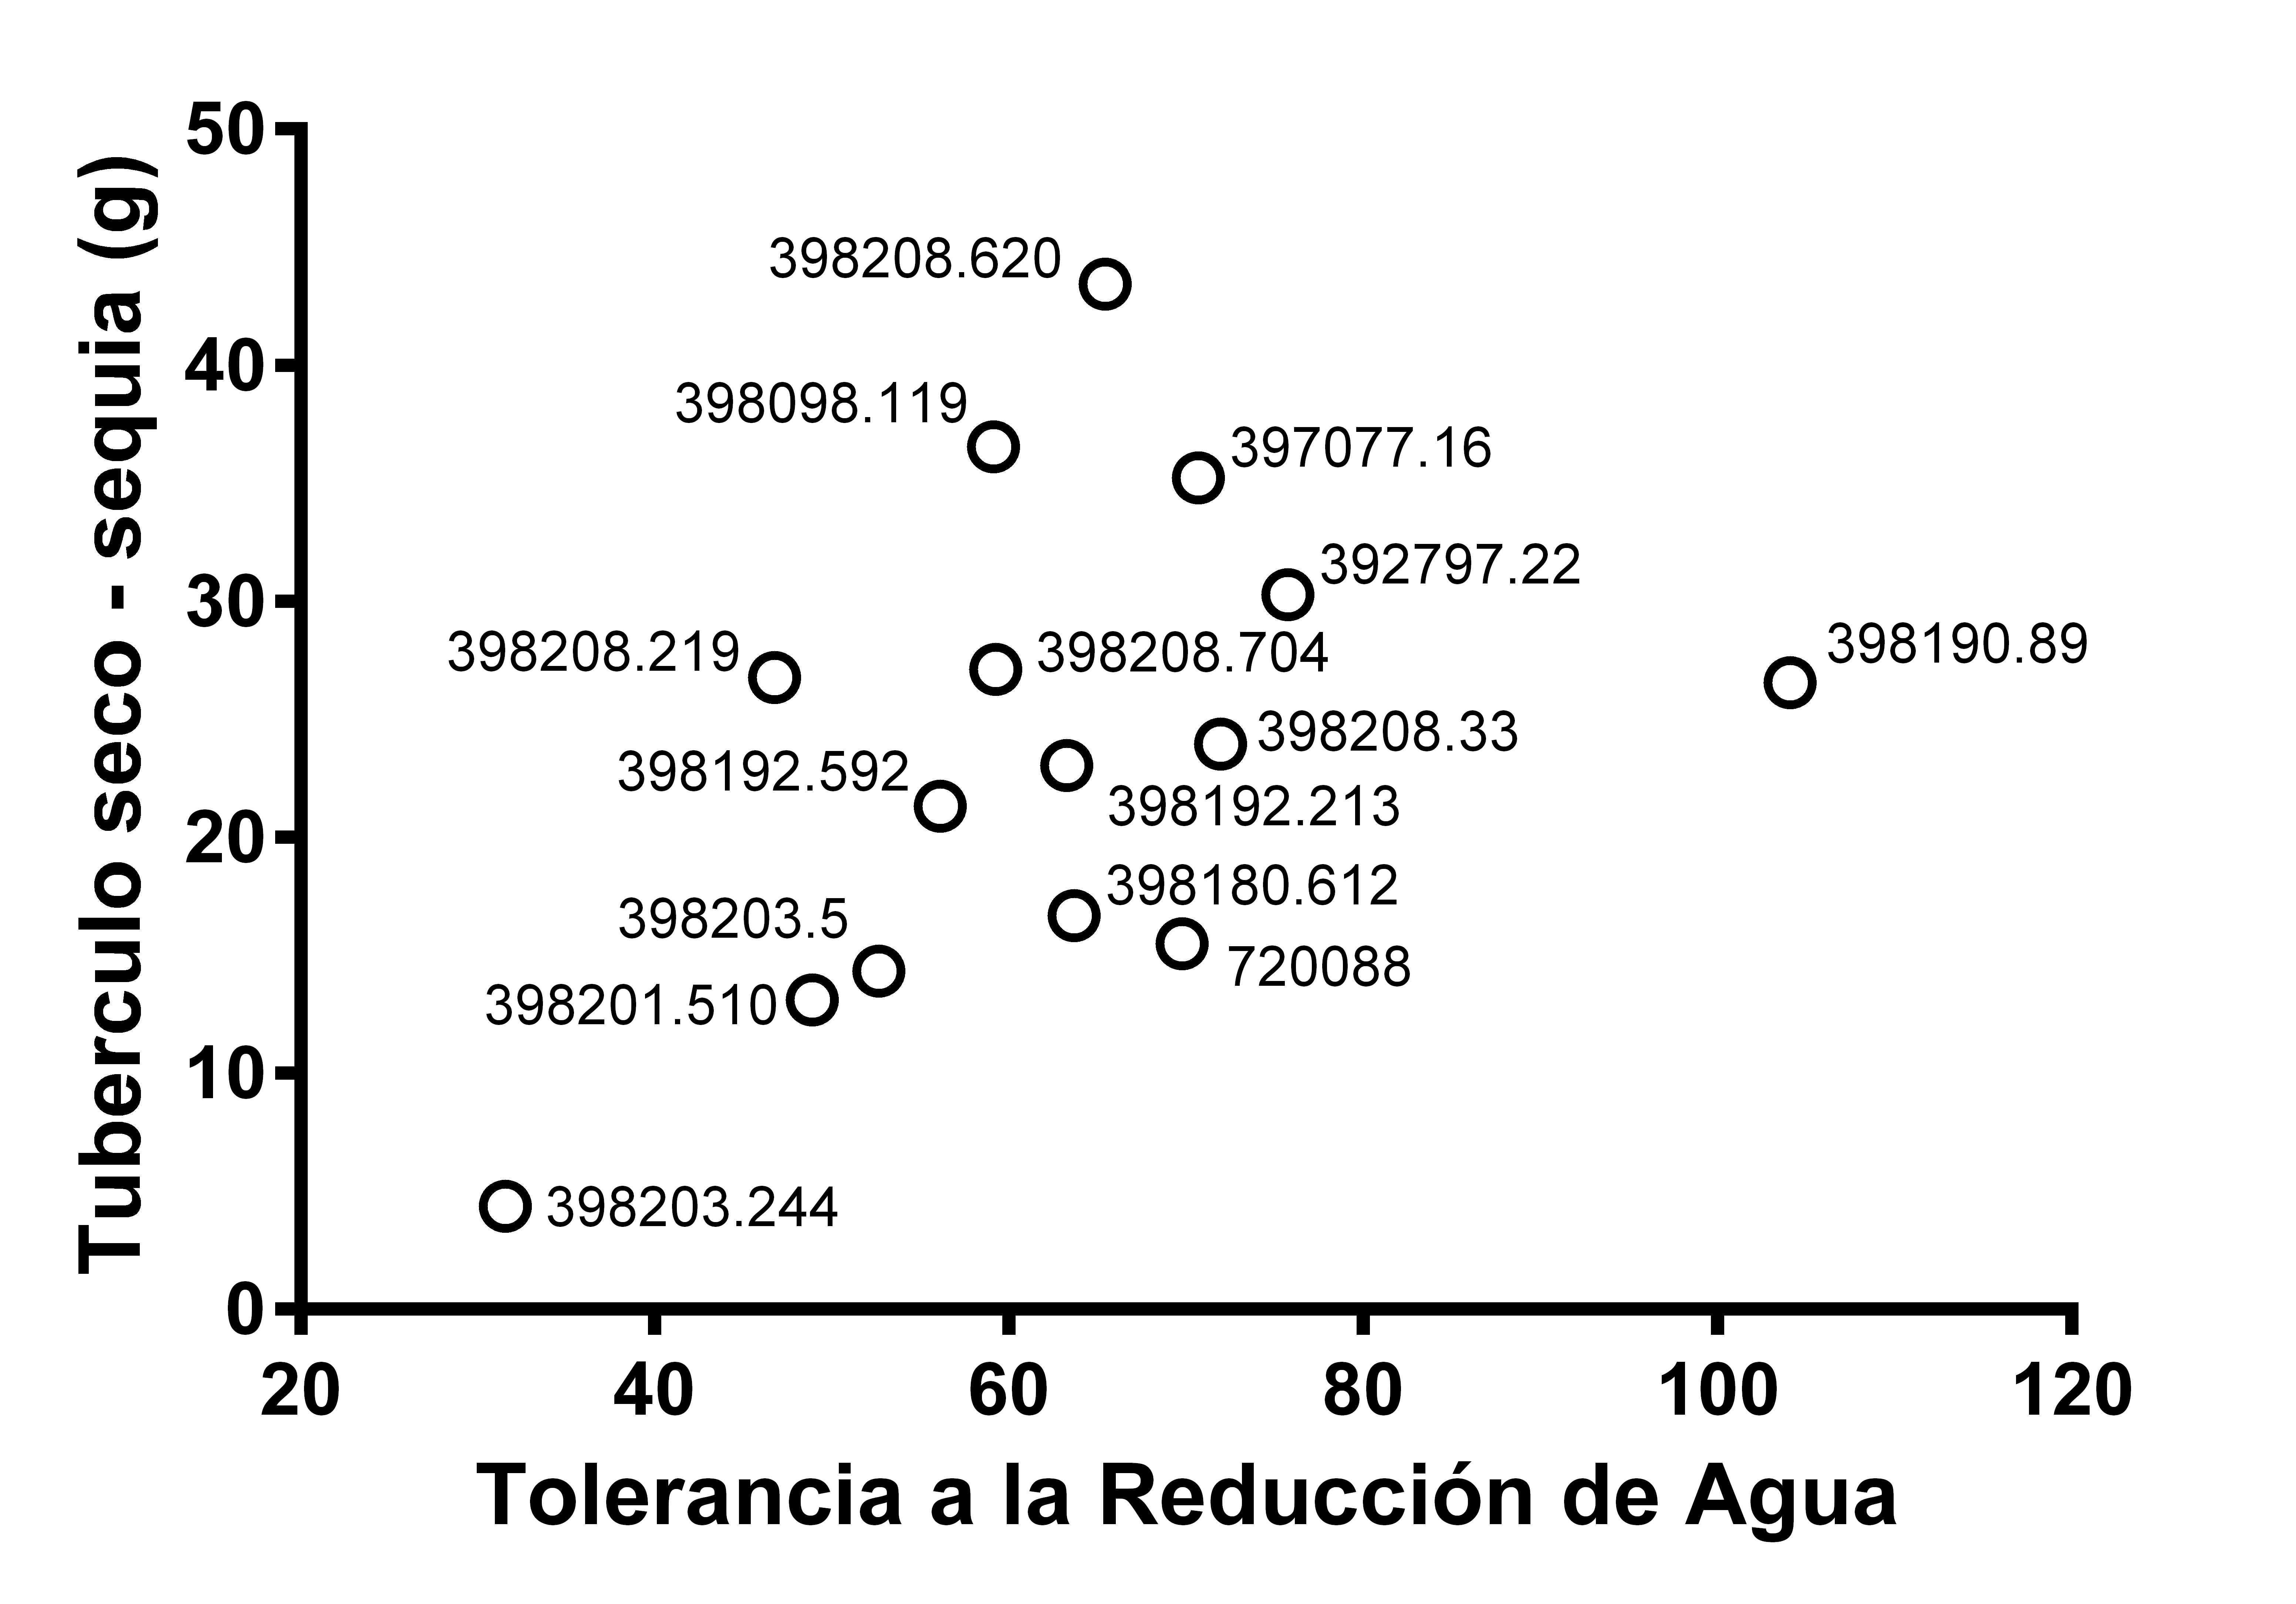
\includegraphics[width=\linewidth]{Tuber-TRA}
\caption{Selecci\'on de clones en base al peso seco de tub\'erculos e \'indice de tolerancia al estr\'es}
\label{fig:yield}
\end{figure}


\begin{figure}[ht]\centering
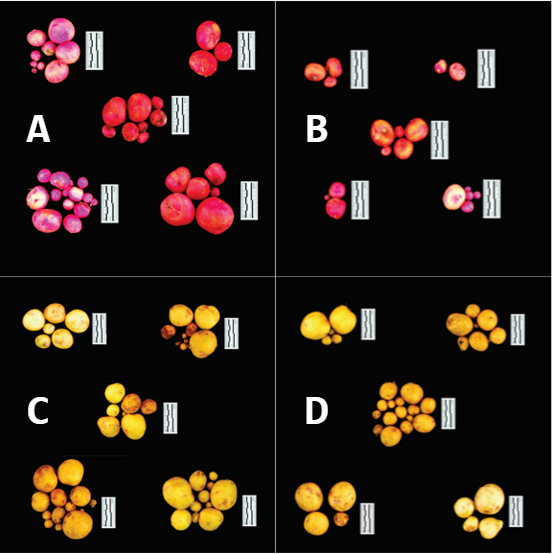
\includegraphics[width=\linewidth]{tubpic}
\caption{Comparaci\'on del rendimiento entre los genotipos CIP398203.244 y CIP398190.89. (A)(C) Plantas sin estr\'es; (B)(D) Plantas con estr\'es}
\label{fig:tpic}
\end{figure}

\subsection{Contenido Relativo de Clorofila}  

El contenido relativo de clorofila a los 29 DDS son similares en entre los tratamientos entre plantas bien regadas y plantas sometidas a estr\'es, esto hace referencia a que las plantas aun no son sometidas al tratamiento de estr\'es y no muestras diferencias entre las mediciones del contenido relativo de clorofila (Fig. \ref{fig:SPAD}). M\'as si existe diferencia entre los genotipos debido que el verdor de las hojas est\'e asociado a caracter\'isticas propias de cada genotipo \citep{THOMAS1993}. A los 83 DDS (38 DDT), se puede notar una disminuci\'on general del contenido relativo de clorofila en los 15 genotipos (Fig. \ref{fig:SPAD}) posiblemente debido a la senescencia de la planta producto de la translocaci\'on de nutrientes. Tambi\'en existe diferencia significativa entre la interacci\'on genotipo por tratamiento ($P<0.05$). Siendo el tratamiento de sequ\'ia regulada el que mantiene valores m\'as altos (44.09 SPAD) que las plantas bajo riego (39.71 SPAD).


\begin{figure}[ht]\centering
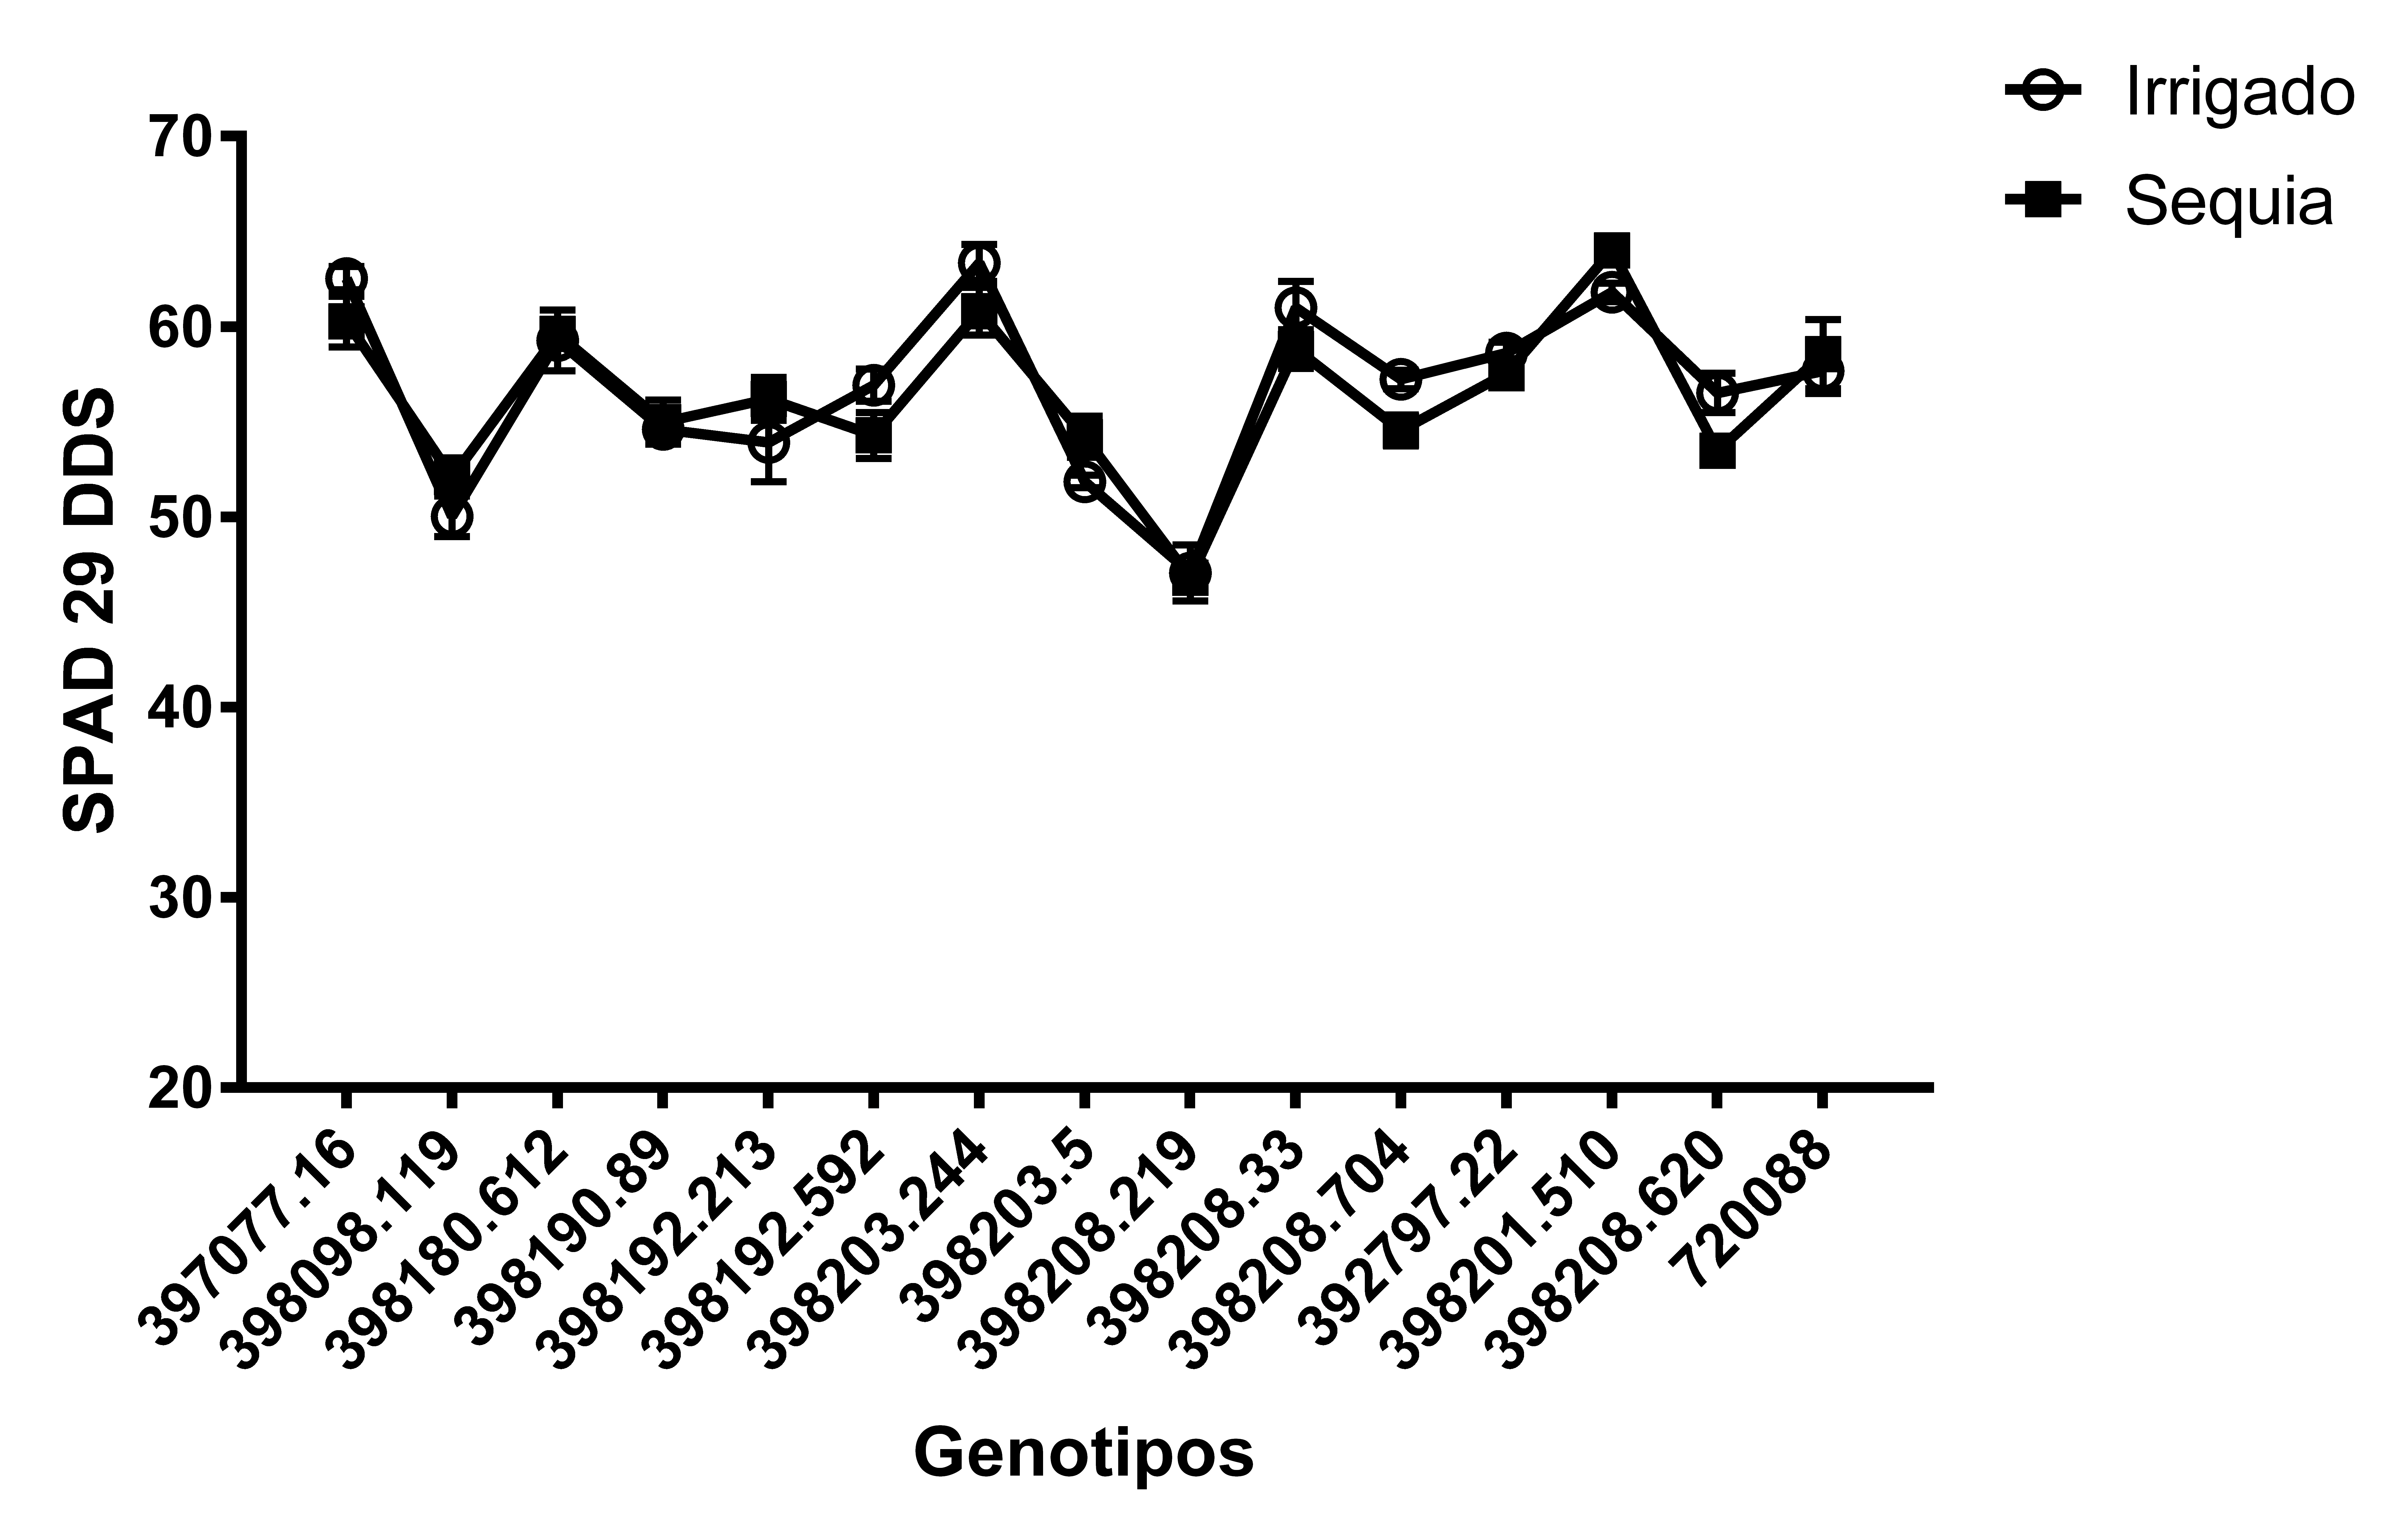
\includegraphics[width=\linewidth]{SPAD29DDS}
\caption{Contenido relativo de clorofila a los a los 29 DDS.}
\label{fig:SPAD}
\end{figure}

\begin{figure}[ht]\centering
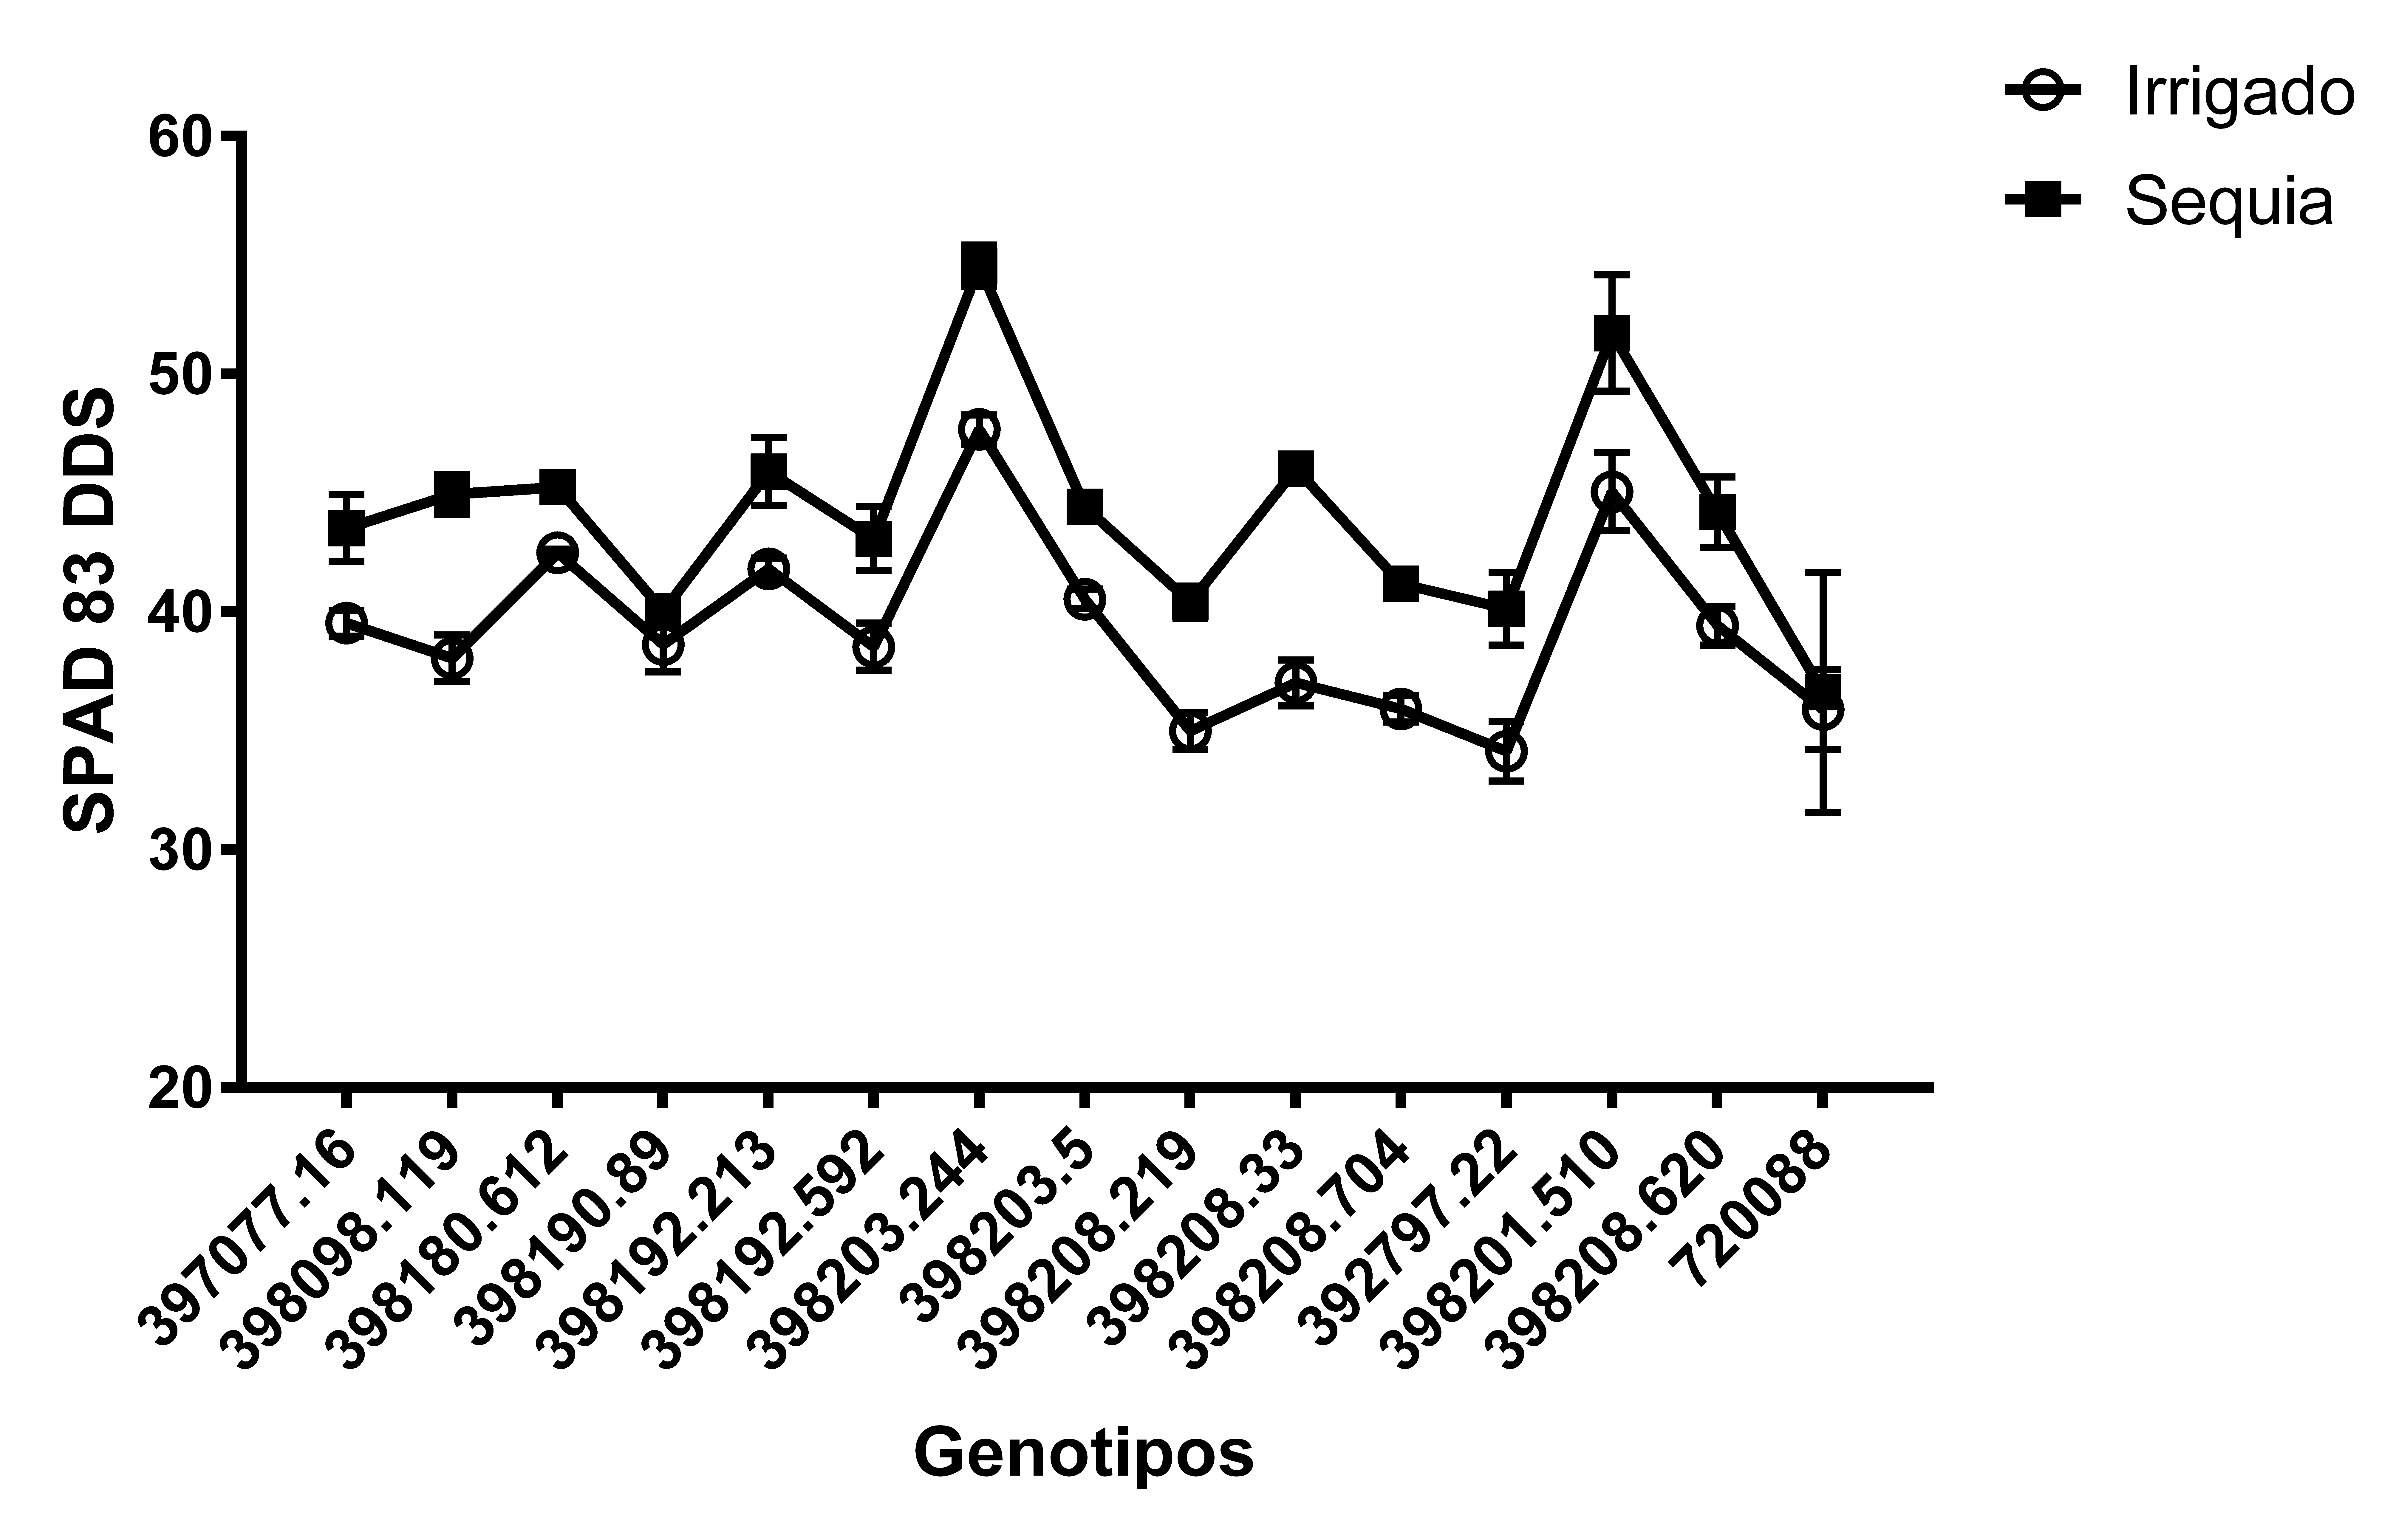
\includegraphics[width=\linewidth]{SPAD83DDS}
\caption{Contenido relativo de clorofila a los a los 83 DDS.}
\label{fig:SPAD2}
\end{figure}

\subsection{Transpiraci\'on total y \'area foliar}

La transpiraci\'on total presenta una interacci\'on genotipo con tratamiento ($p = 0.018$) lo que indica que existe influencia del efecto de la sequ\'ia regulada sobre las plantas en donde las plantas que presentaron mayor transpiraci\'on fueron las plantas bien regadas. Los clones con mayor transpiraci\'on bajo condiciones de riego fueron los genotipos CIP398098.119 con 10.43 l ; CIP398208.219 con 9.99 l y  CIP398192.592 con  9.54 l. Y los genotipos que tuvieron una tasa mayor de transpiraci\'on en sequ\'ia regulada fueron los genotipos CIP398098.119 con 6.29 l; CIP398208.620 con 5.47 l y CIP398192.592 con 5.33 l. Tambi\'en se observa un comportamiento at\'ipico del genotipo CIP720088, que tanto en condiciones de riego y de sequ\'ia controlada posee una tasa baja de transpiraci\'on, 3.37 l y 2.33 l respectivamente (Fig. \ref{fig:Trans}). En el an\'alisis de \'area foliar, se observa una interacci\'on significativa del tratamiento sobre los genotipos estudiados ($p < 0.001$). Lo que nos indica que las plantas de papa responden a la sequ\'ia con cambios en el \'area foliar. Los genotipos en riego que presentaron mayor \'area foliar fueron CIP398098.119 con 10287.8 $cm^2$ ; CIP398208.219  con 9669 $cm^2$ y CIP398208.704 con 8878.8 $cm^2$. Y el genotipo CIP720088 presenta un comportamiento at\'ipico ya que su \'area foliar en sequ\'ia regulada como riego presenta \'area foliar reducida  680.6 y 1374 $cm^2$ respectivamente (Fig. \ref{fig:AF}).

\begin{figure}[ht]\centering
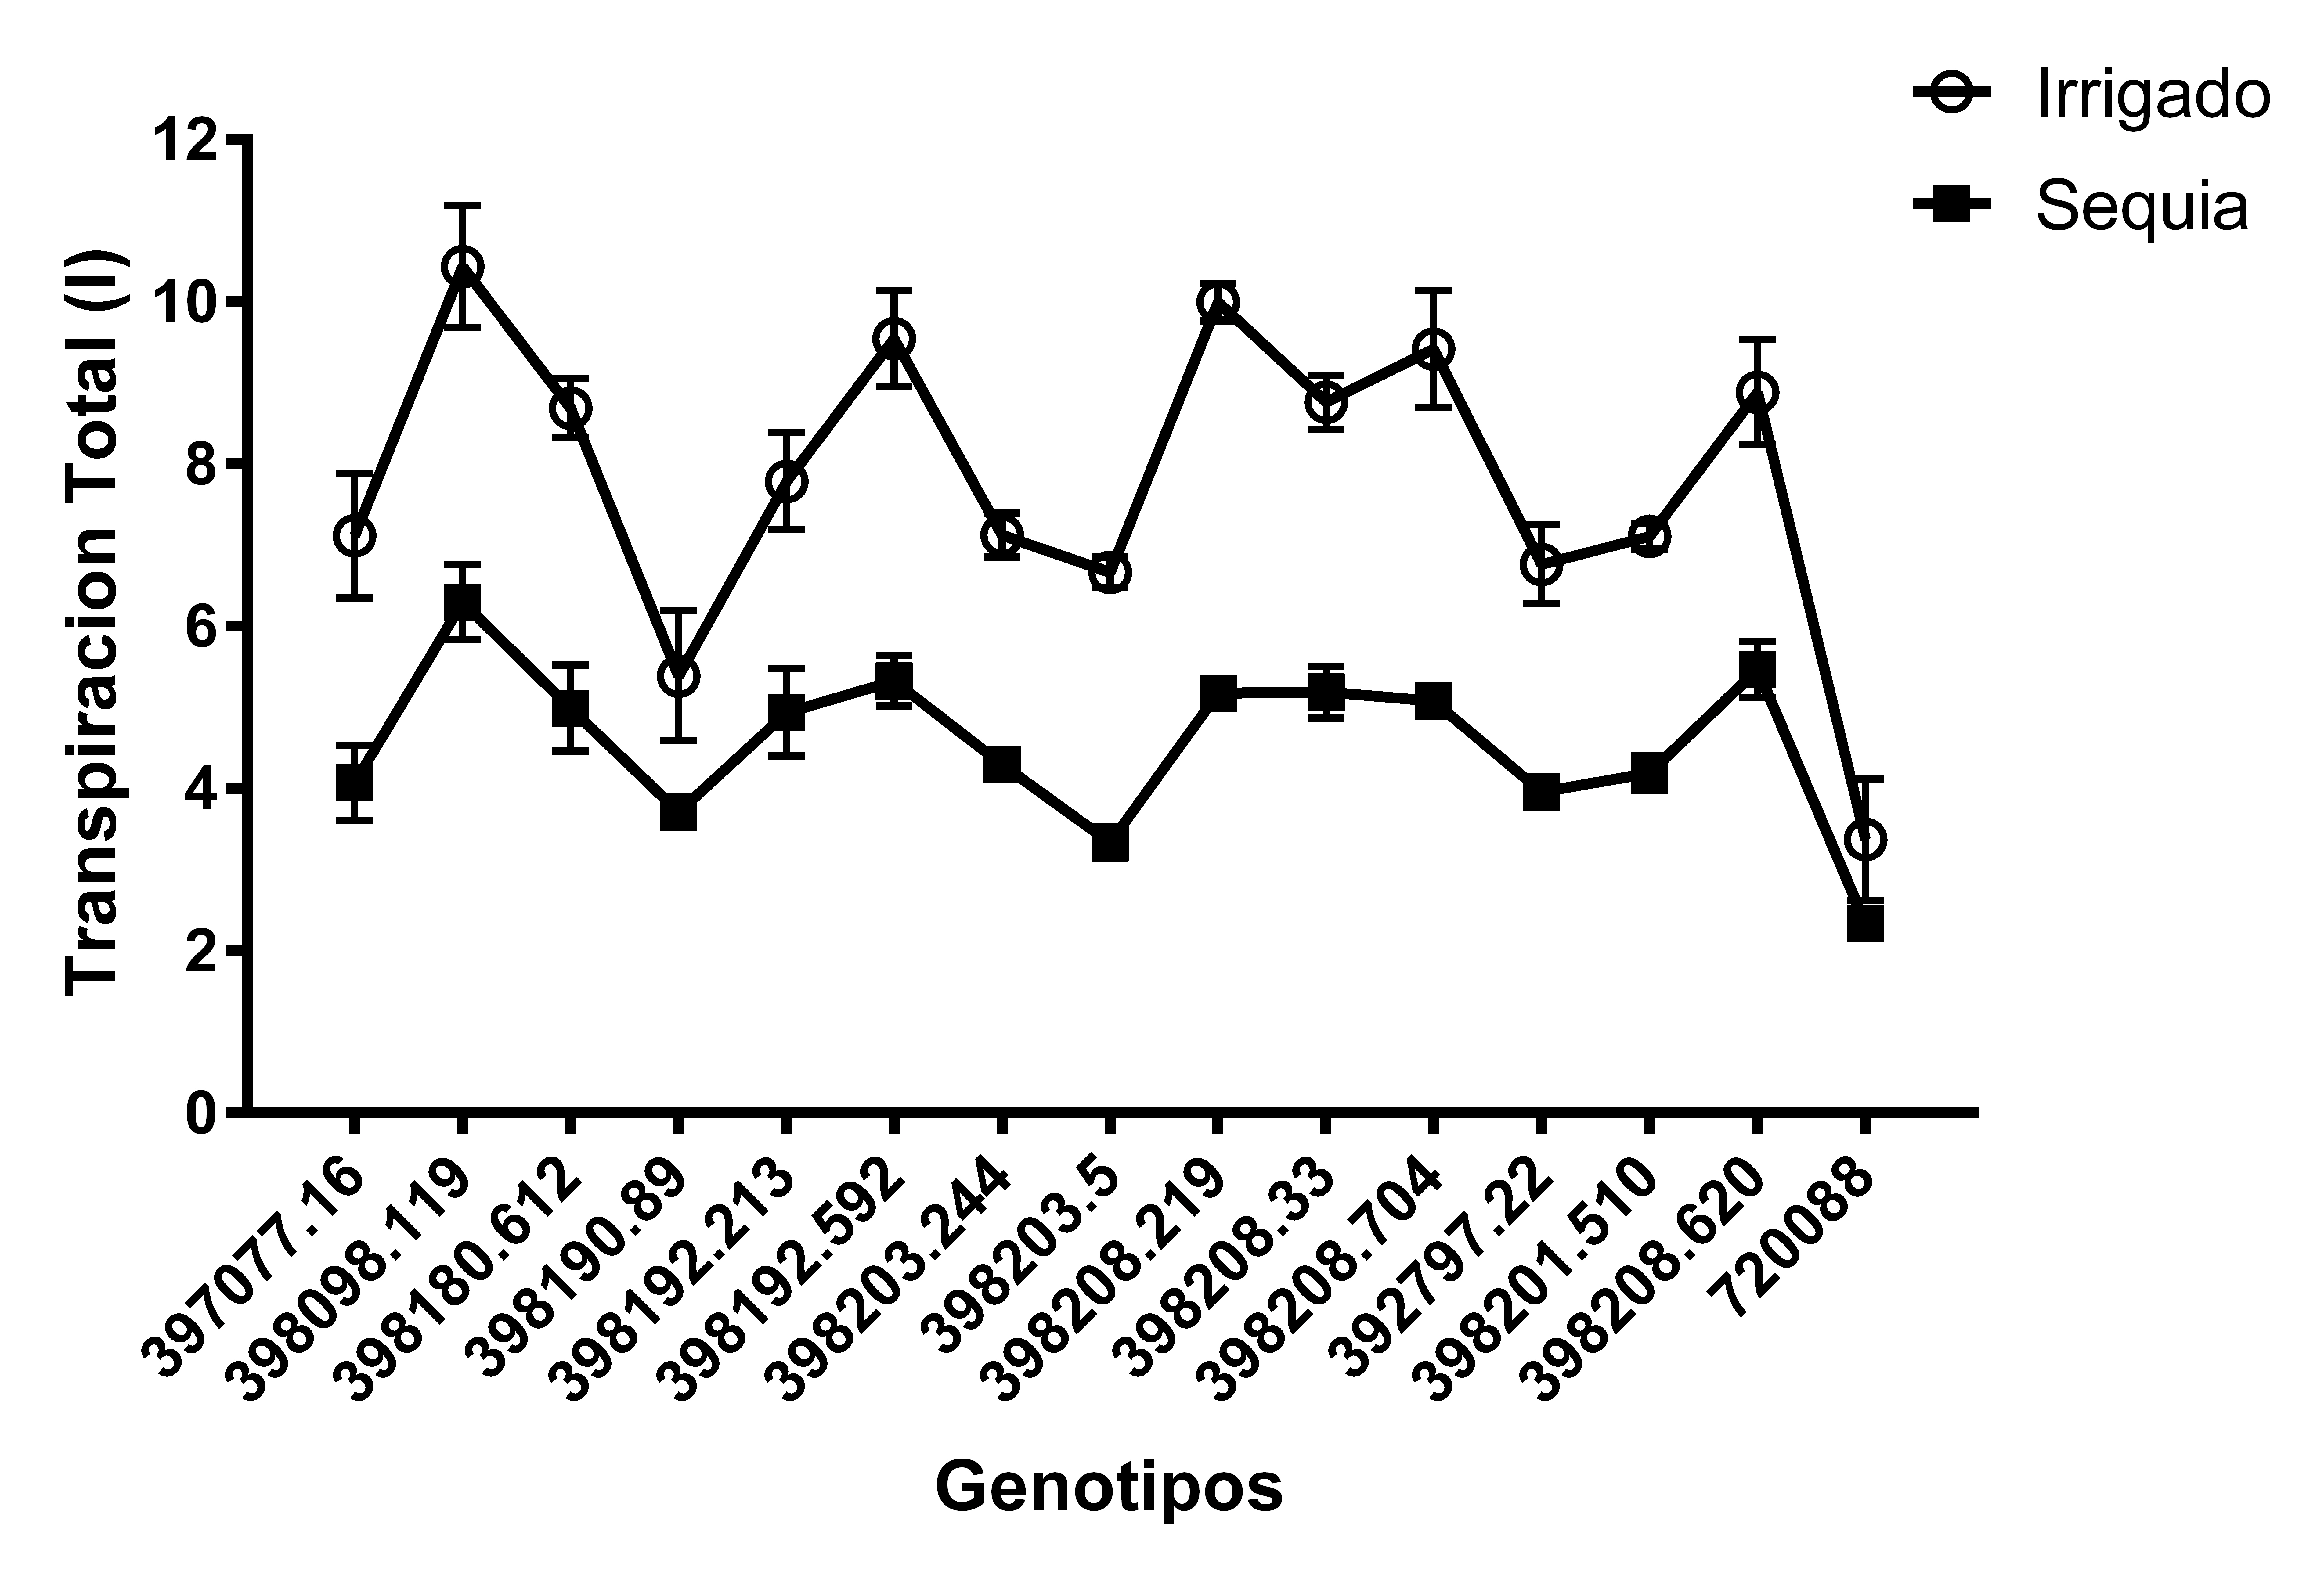
\includegraphics[width=\linewidth]{Transpiracion}
\caption{Transpiraci\'on Total}
\label{fig:Trans}
\end{figure}

\begin{figure}[ht]\centering
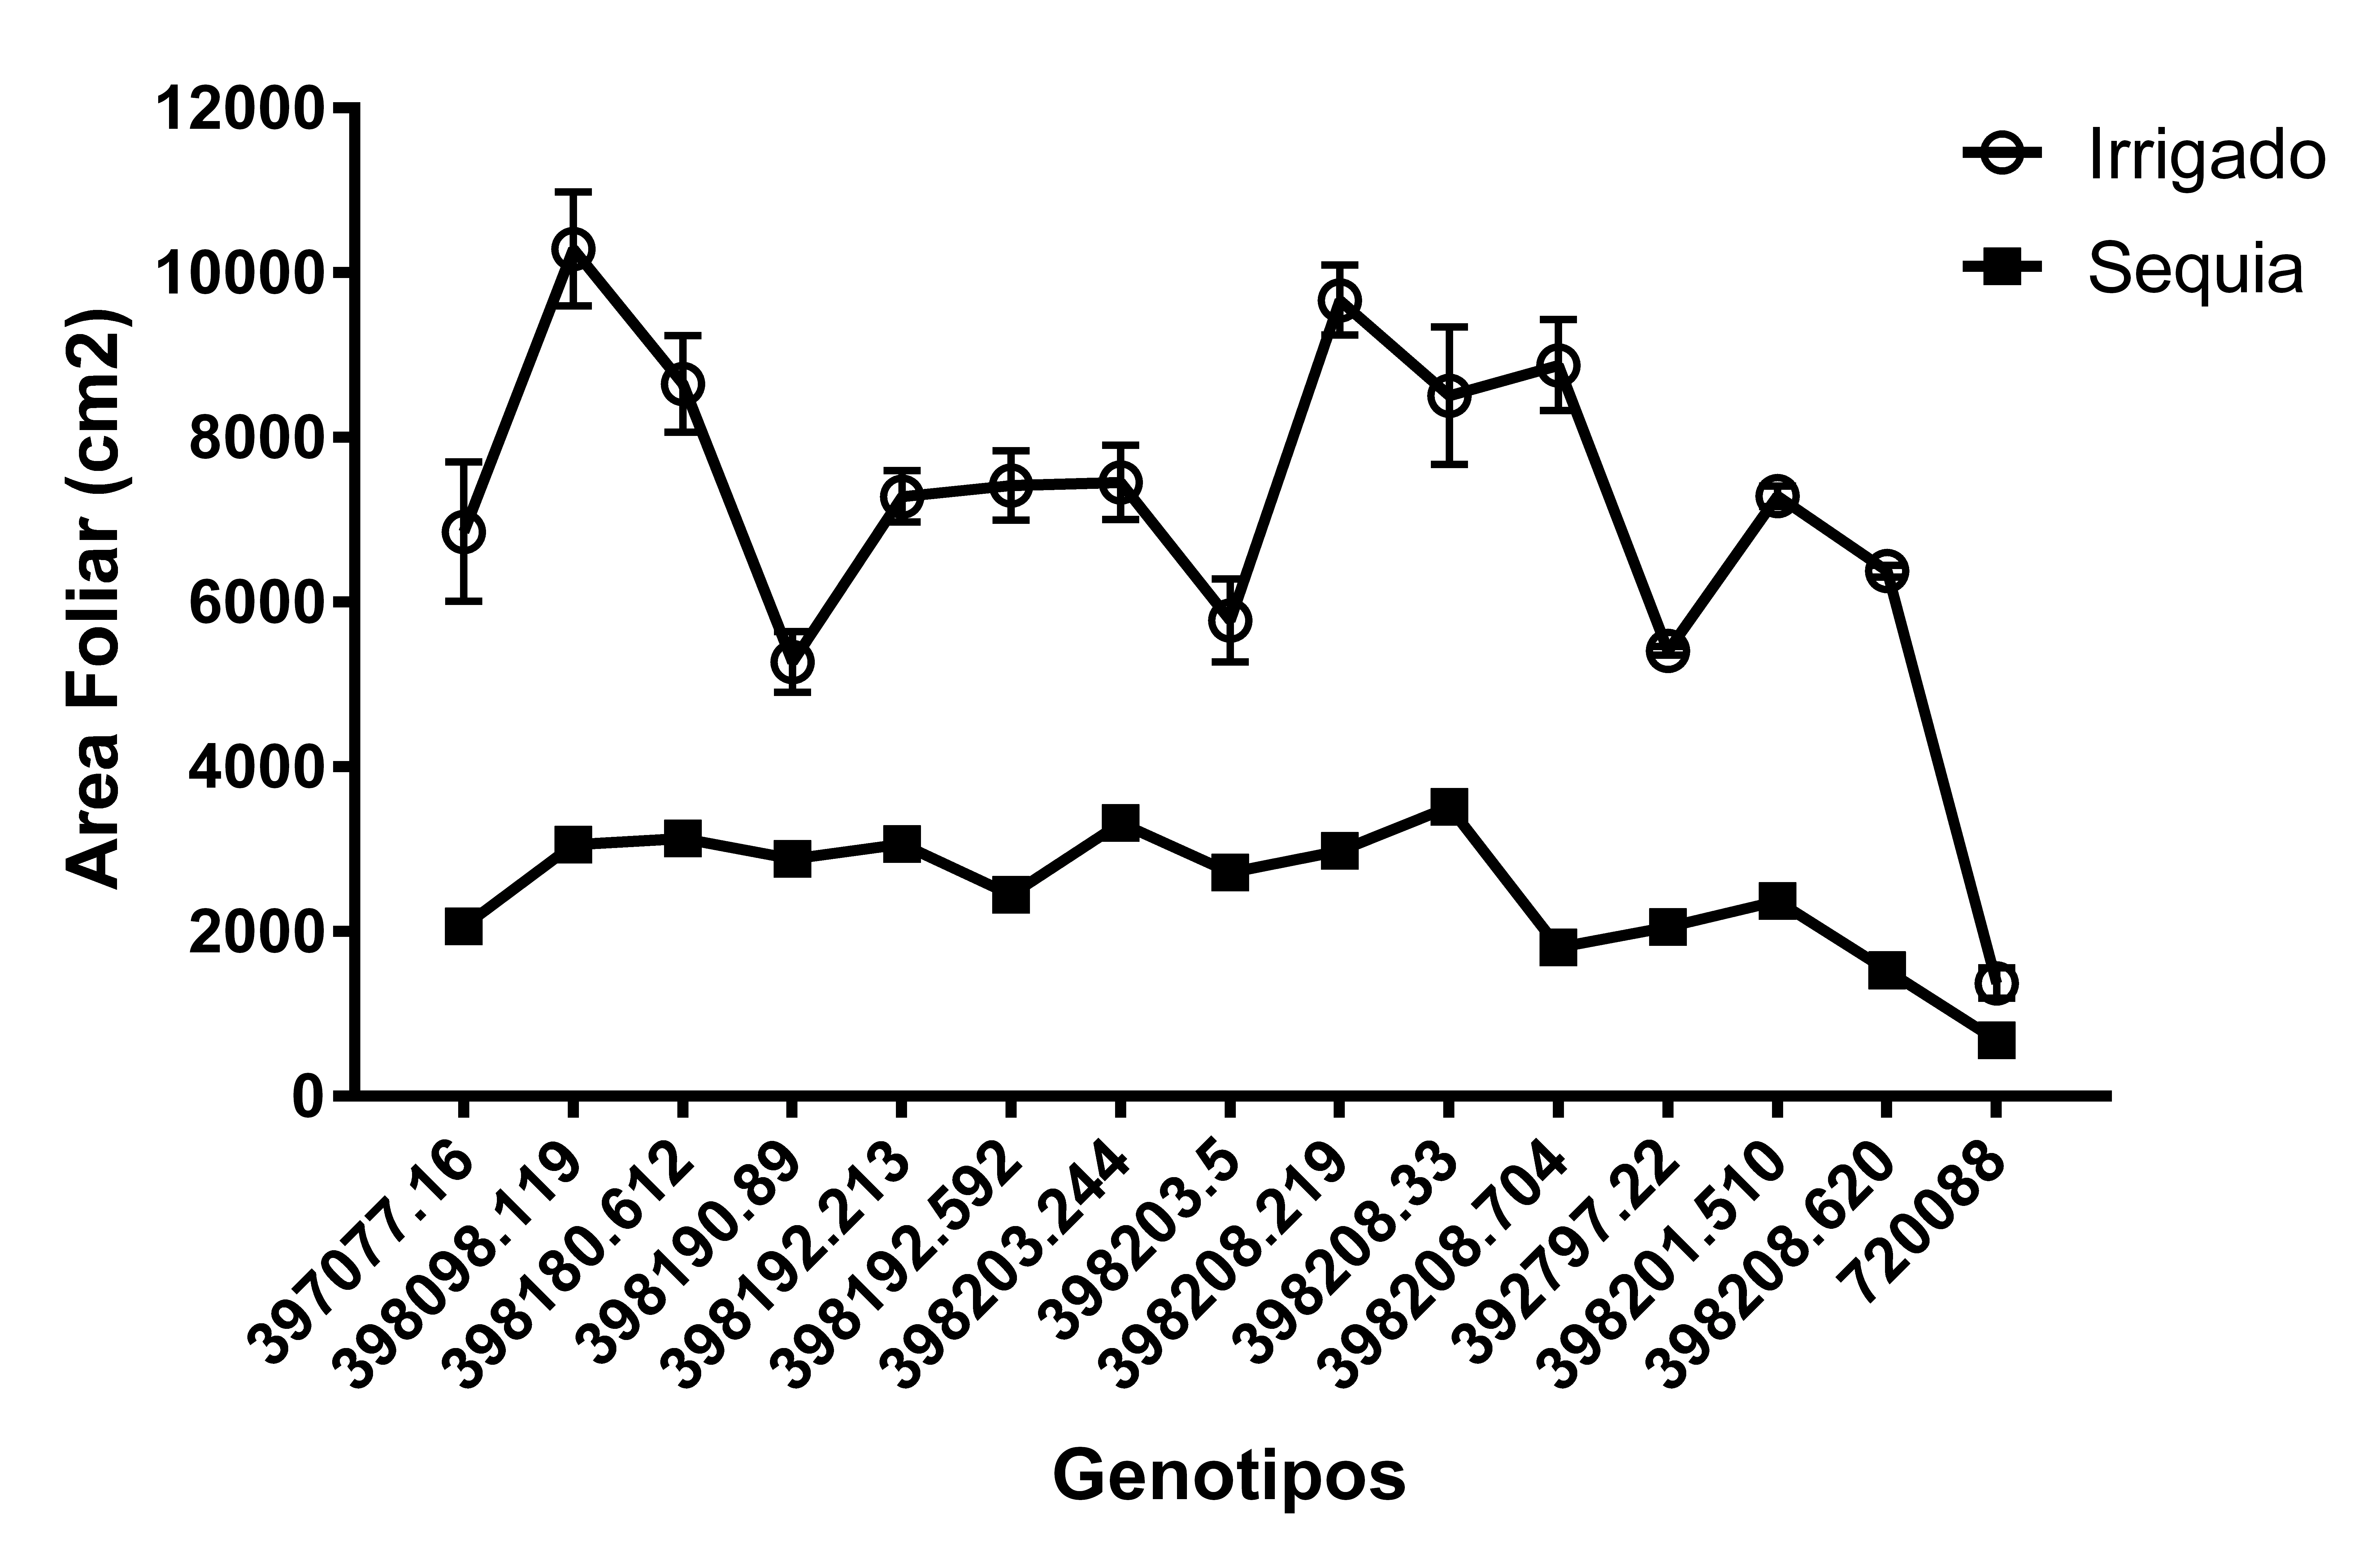
\includegraphics[width=\linewidth]{AF}
\caption{\'Area Foliar}
\label{fig:AF}
\end{figure}

\subsection{Eficiencia de Uso de Agua en la biomasa y tub\'erculos} 	

De acuerdo a los resultados no que existe diferencia significativa entre tratamientos ($p = 0.08$) para la eficiencia de uso de agua en tub\'erculo ($EUA_T$) mas si entre genotipos con ($p < 0.001$) \citep{Anyia2004} . Los genotipos que presentaron mayor EUAT fueron CIP397077.16 con  7.95 $g/l$; CIP398208.620  con  7.34 $g/l$ y CIP392797.22 con  7.31 $g/l$. Los genotipos que presentaron los valores m\'as bajos en EUAT fueron CIP398201.510 con 3.54 $g/l$ ; CIP398180.612 con 3.19 $g/l$ y CIP398203.244 con 1.53 $g/l$ (Fig. \ref{fig:EUAt}). Para le eficiencia de uso de agua en relaci\'on a la biomasa, existe diferencia significativa tanto para los tratamientos y los genotipos con $p = 0.002$ y $p < 0.001$ respectivamente . El promedio para el tratamiento de sequ\'ia regulada fue 11.12 $g/l$ y 9.41 $g/l$ para las plantas bien regadas. Los genotipos que presentaron mayor EUA fueron los genotipos CIP397077.16 con  12.51 $g/l$; CIP392797.22 con 12.04 $g/l$ y CIP398208.620 con 11.51 $g/l$ y los genotipos que presentaron los valores m\'as bajos fueron CIP720088 con   9.37 $g/l$ ; CIP398201.510 con 9.29 $g/l$ y CIP398180.612 con 9.17 $g/l$ Fig. \ref{fig:EUAb}).

\begin{figure}[ht]\centering
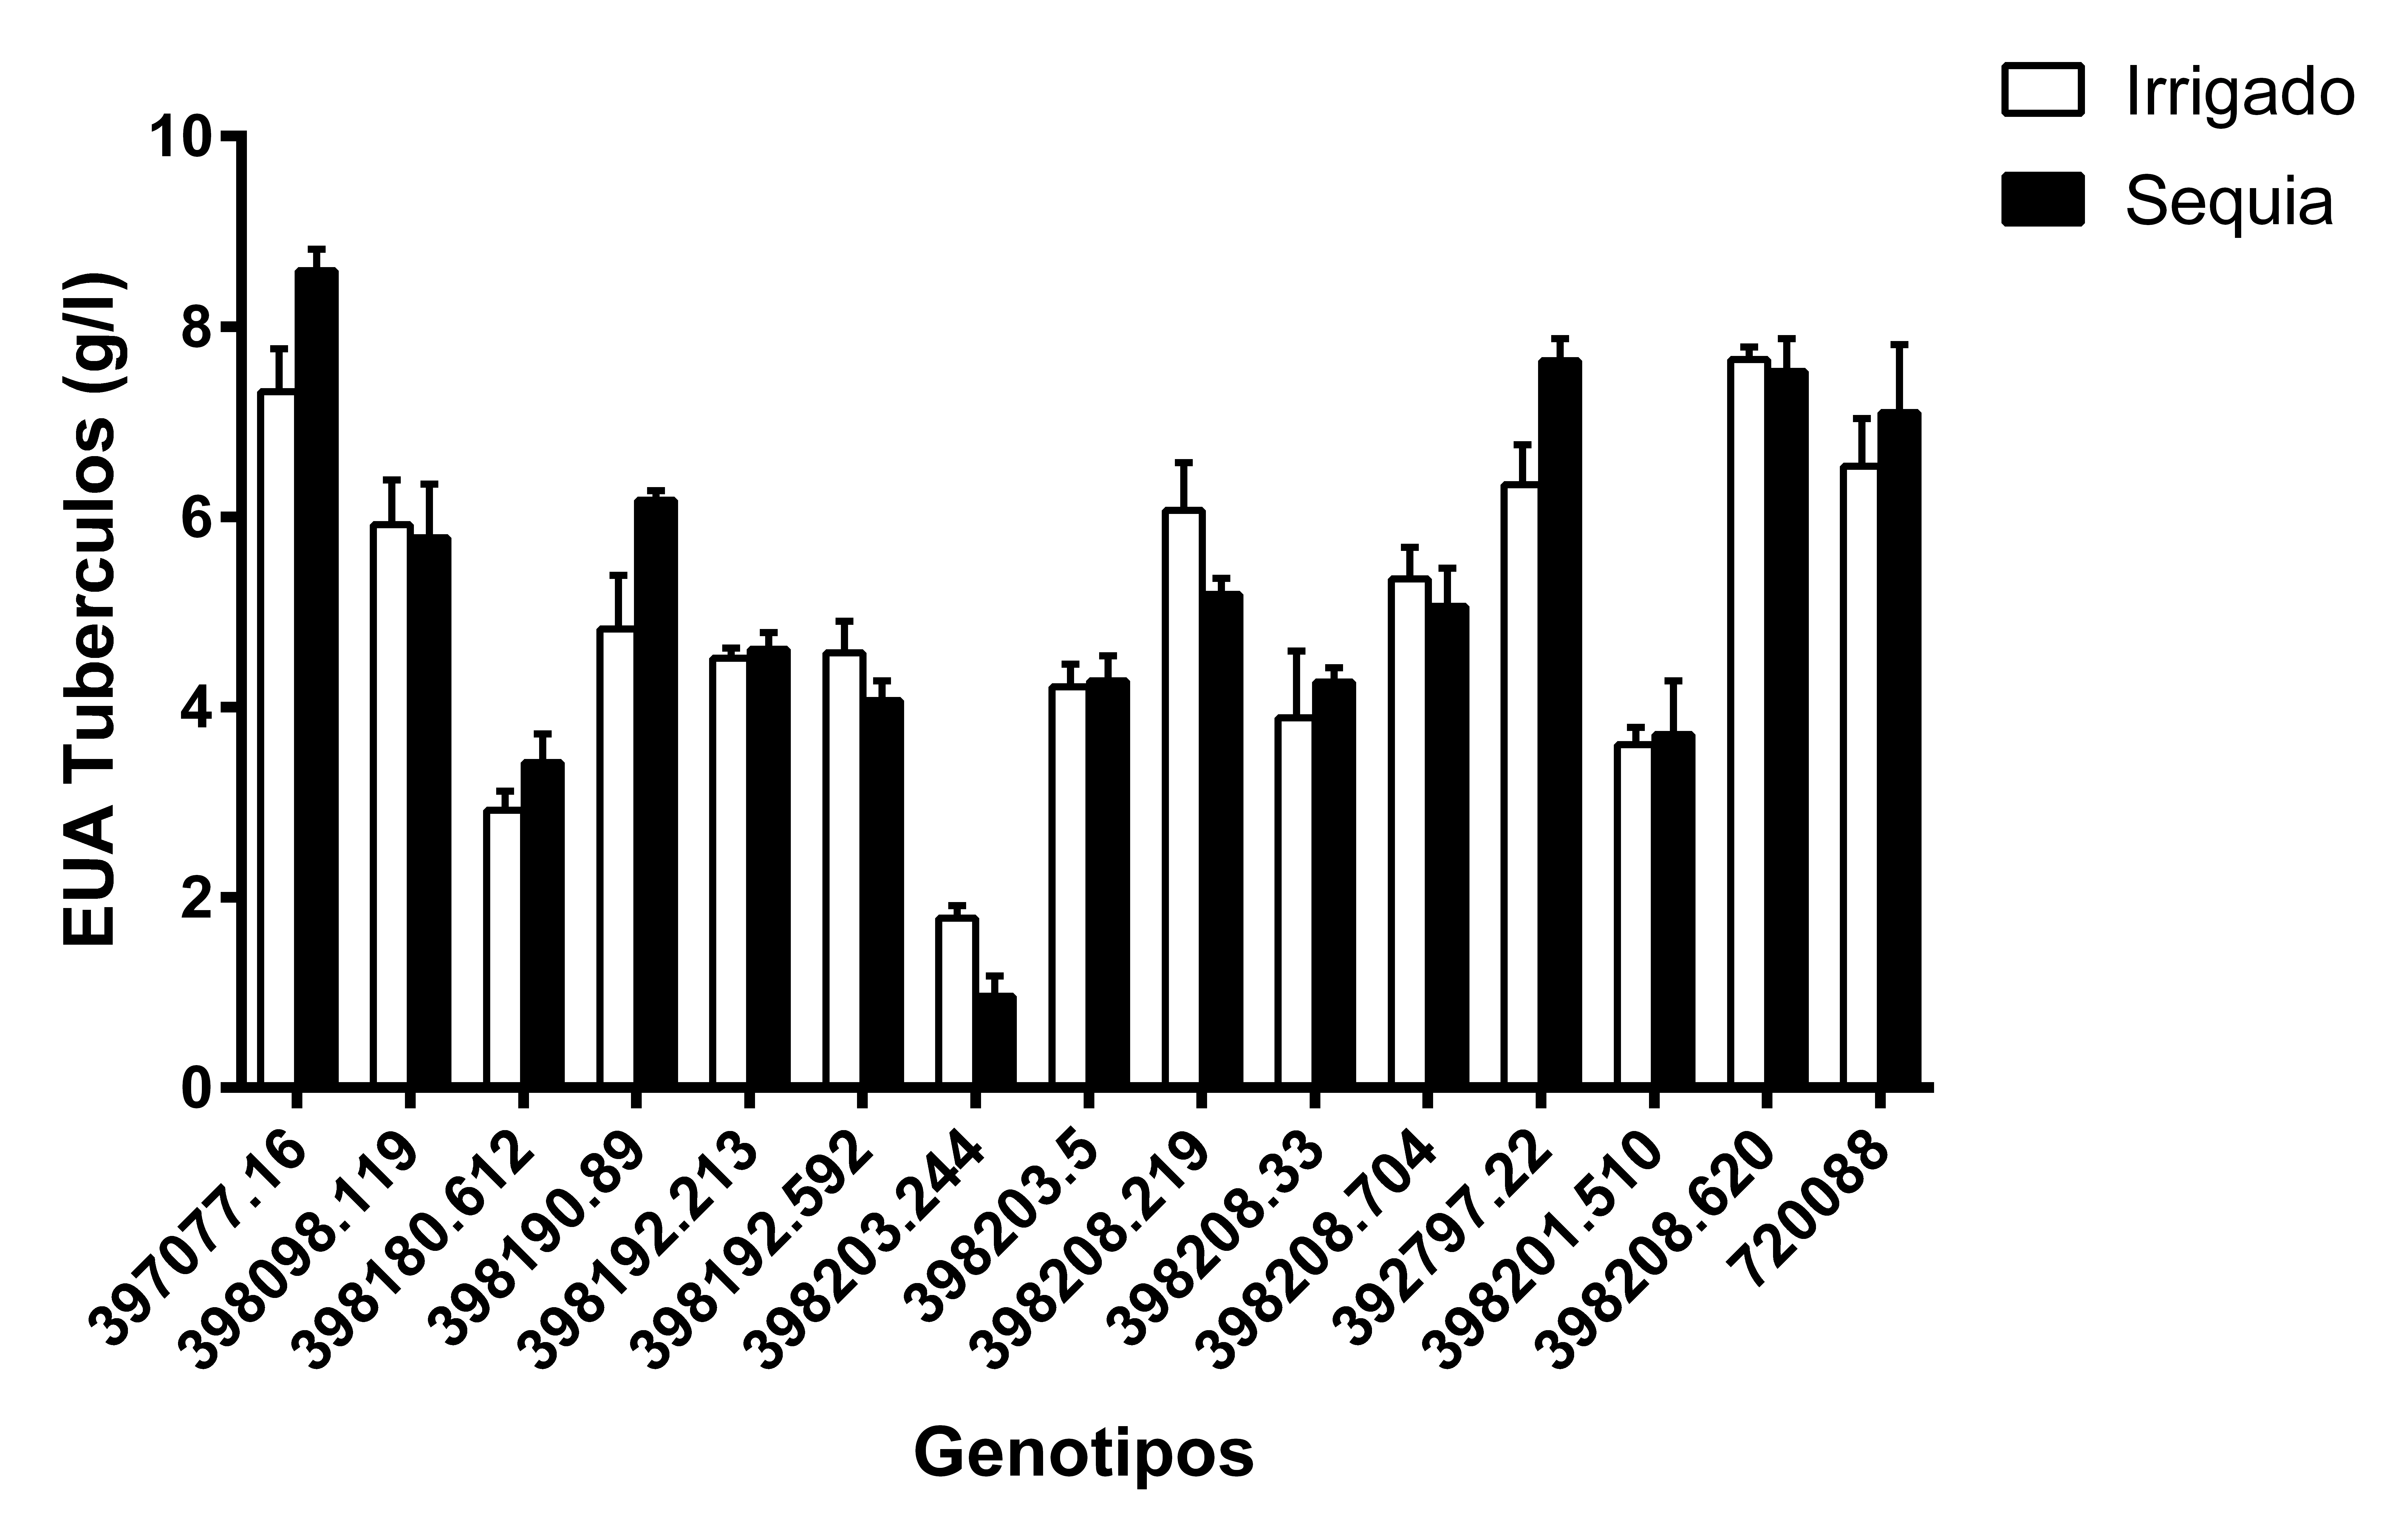
\includegraphics[width=\linewidth]{EUAtub}
\caption{Eficiencia de uso de agua en tub\'erculos}
\label{fig:EUAt}
\end{figure}

\begin{figure}[ht]\centering
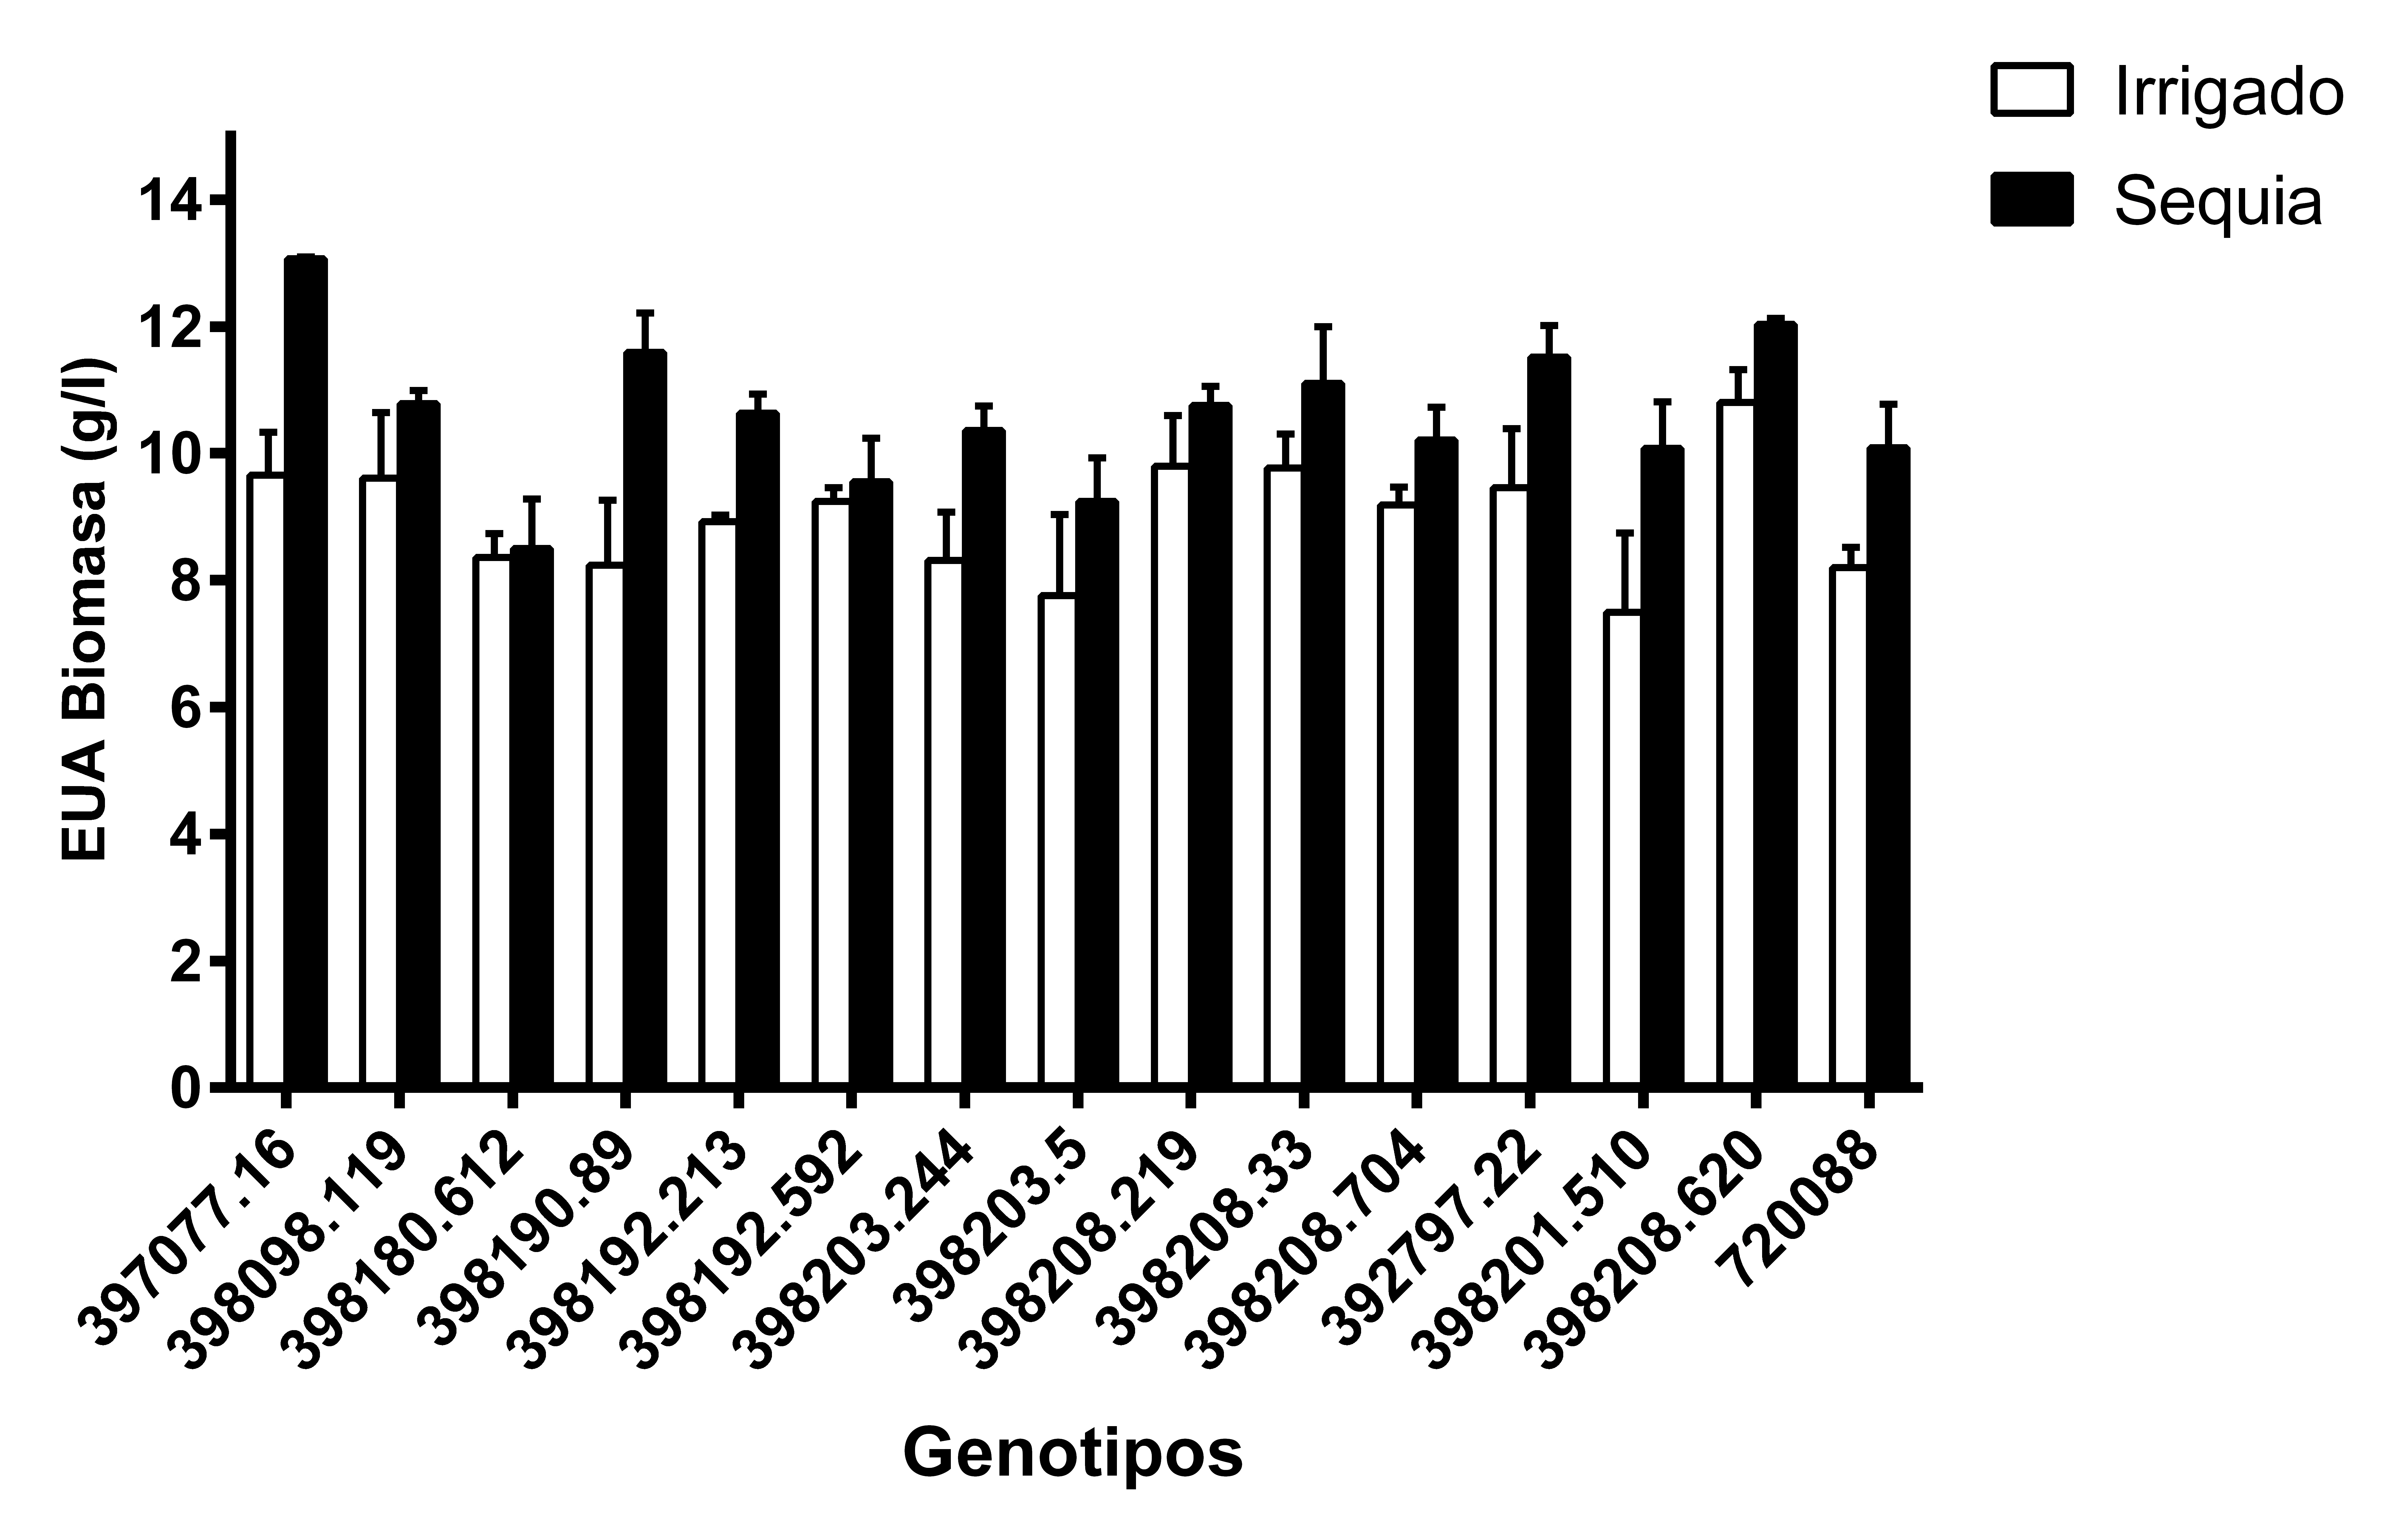
\includegraphics[width=\linewidth]{EUAbiom}
\caption{Eficiencia de uso de agua en  biomasa}
\label{fig:EUAb}
\end{figure}

\subsection{Eficiencia de Uso de Agua en tub\'erculos e \'indice de Cosecha}

La eficiencia de uso de agua en tub\'erculos ($g/l$) posee una correlaci\'on alta con el \'indice de cosecha ($r = 0.912$) (Fig. \ref{fig:TDWS2}) . Adicionalmente el peso seco de la biomasa tiene correlaci\'on alta con la transpiraci\'on total $r = 0.928$ ($p < 0.001$).


\begin{figure}[ht]\centering
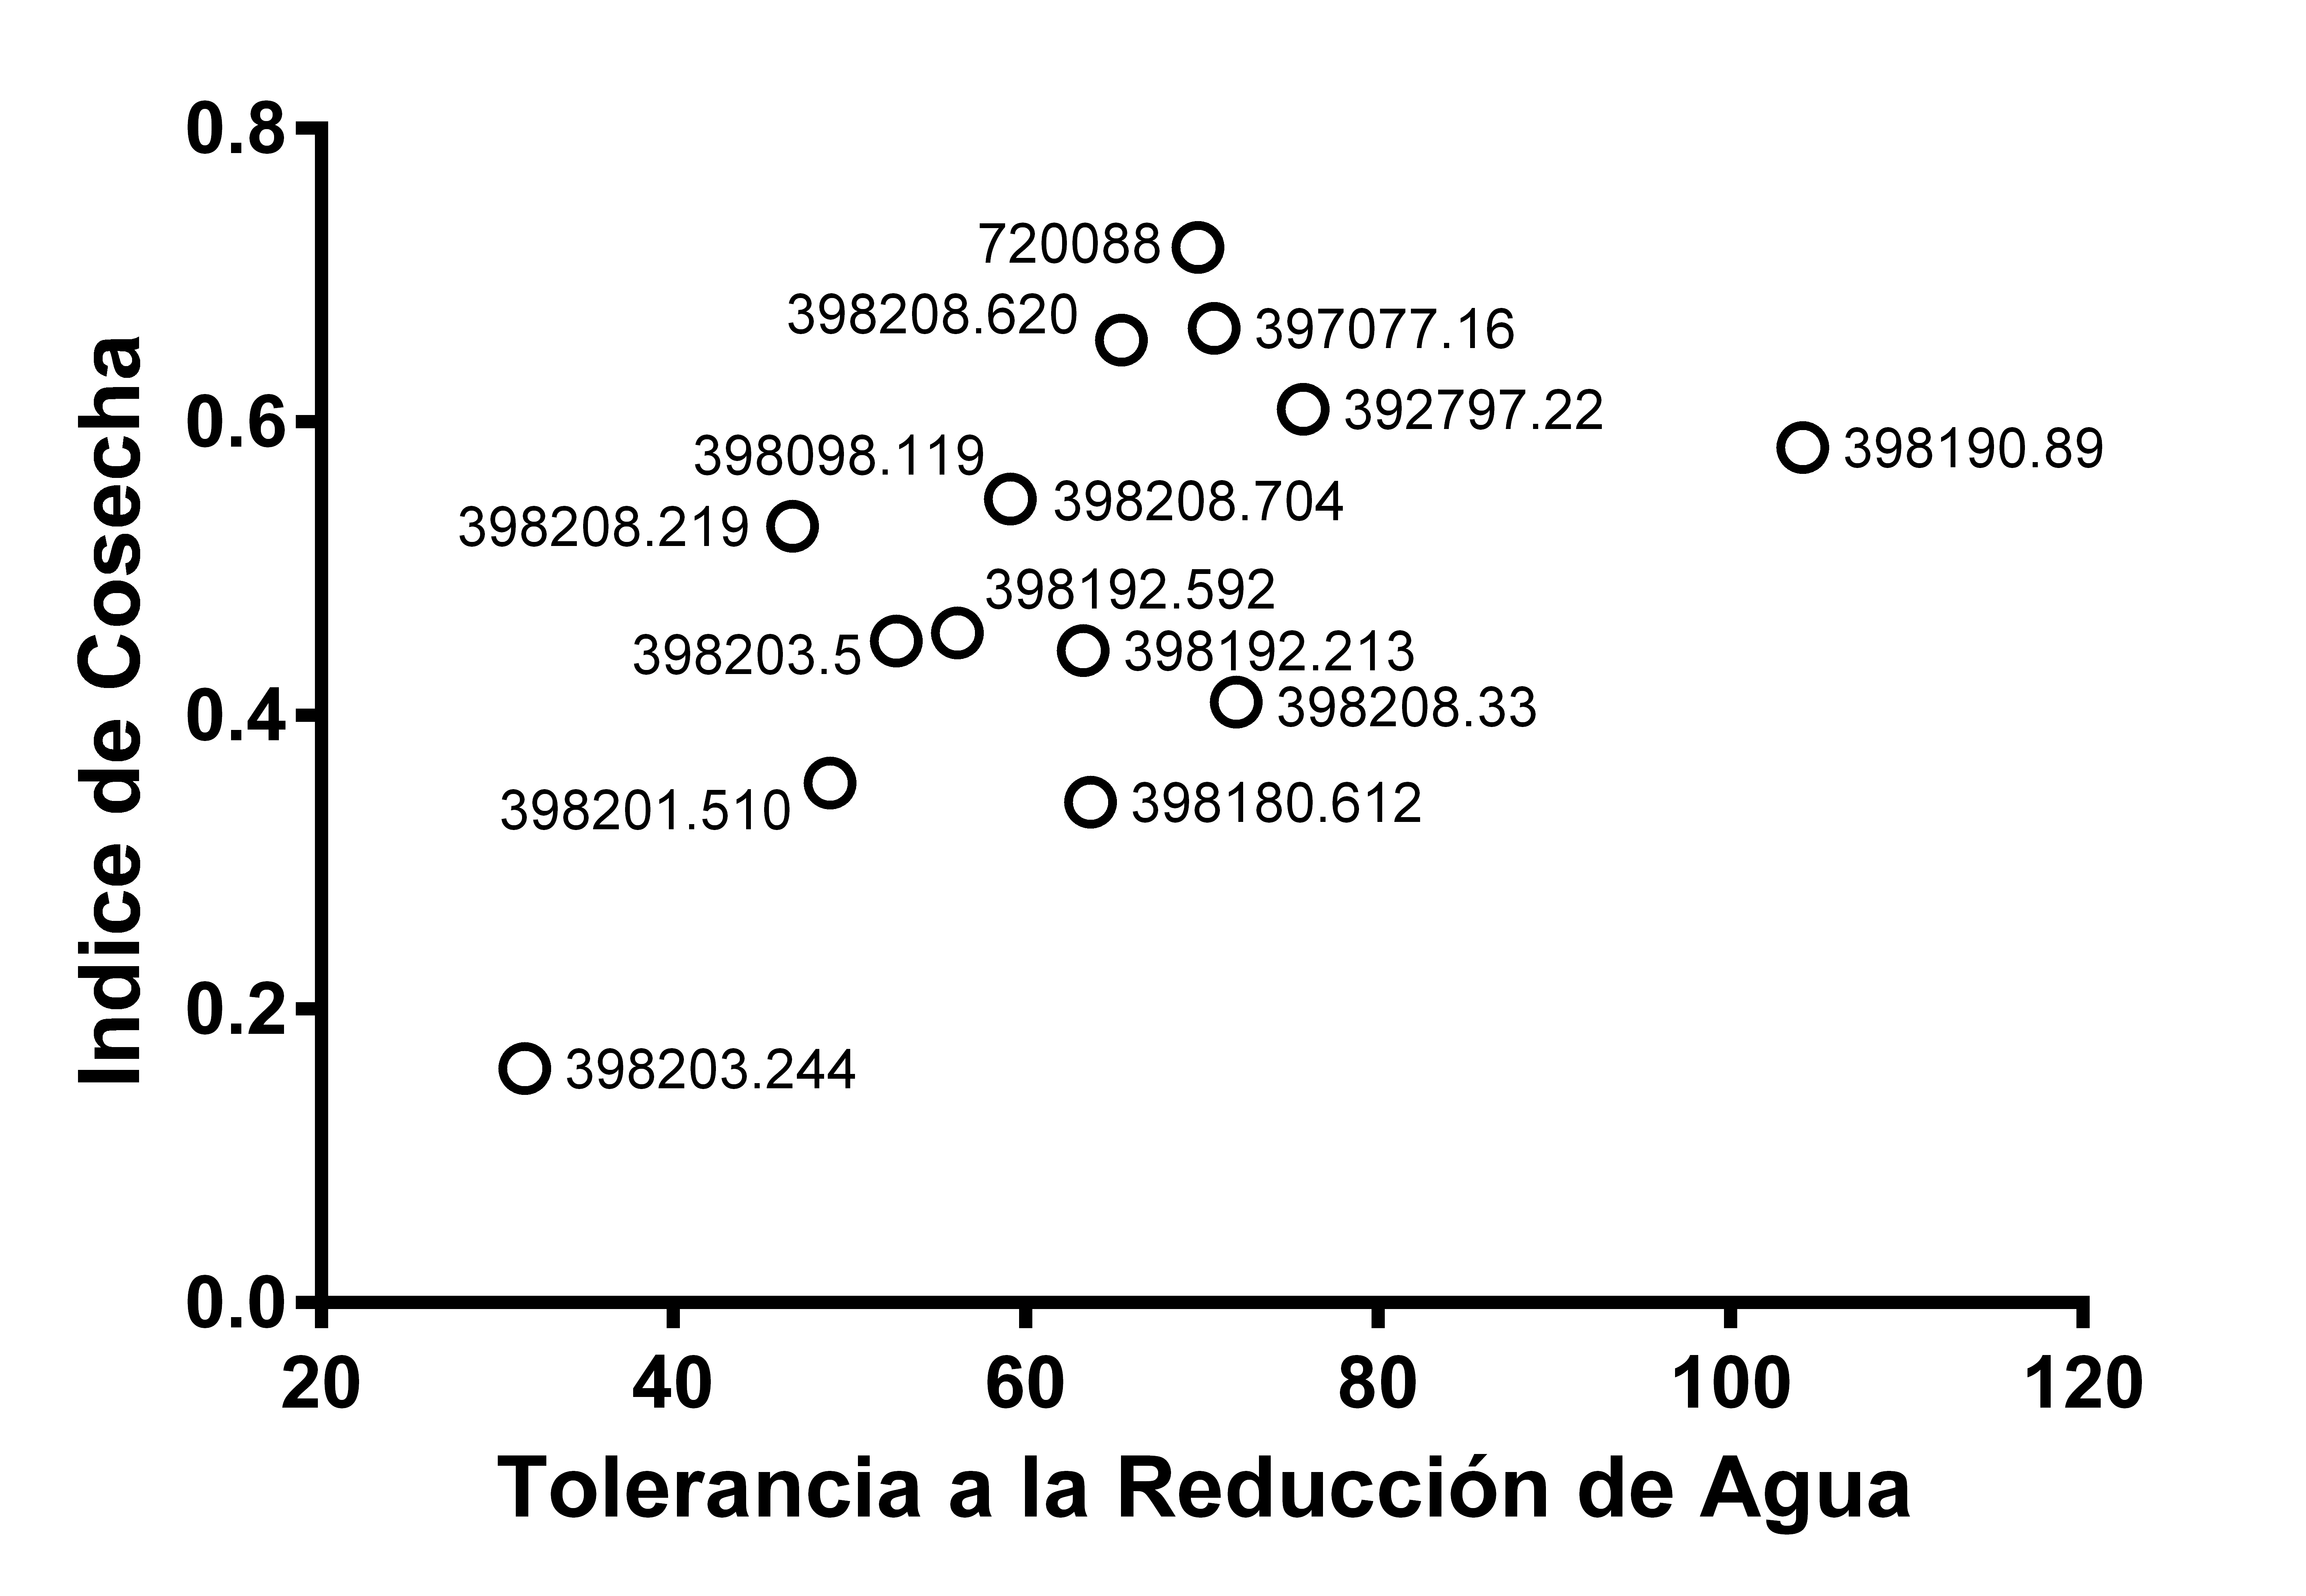
\includegraphics[width=\linewidth]{TRA-IC}
\caption{Clones con tolerancia al estr\'es por sequ\'ia en base al \'indice de cosecha}
\label{fig:TDWS2}
\end{figure}

\section{Discusi\'on}

El rendimiento bajo condiciones manejadas de estr\'es puede predecir el rendimiento en condiciones naturales (campo). Ganancia bajo esta selecci\'on ha sido demostrado con anterioridad \citep{IRRI18/06/14}.El efecto de la sequ\'ia en el rendimiento depender\'a del estado de desarrollo del cultivo la intensidad y duraci\'on al estr\'es por reducci\'on del agua \citep{Kumar1994}. En la agricultura de subsistencia, un rendimiento estable es m\'as importante que un rendimiento alto en ambientes favorables. En la agricultura comercial,  altos rendimientos son altos ingresos lo cual es el objetivo deseado \citep{Rosielle1981}. La combinaci\'on de altos rendimientos estables y altos rendimientos en sequ\'ia, ha sido propuesto como un criterio de selecci\'on para caracterizar el desempe\~no del genotipos bajo distintos grados de variaci\'on en la sequ\'ia \citep{AHMAD2003}, ya que la sequ\'ia es un fen\'omeno err\'atico e impredecible, el objetivo de los mejoradores es mejorar la capacidad de las plantas a la tolerancia al estr\'es por sequ\'ia mientras mantengan a su vez un rendimiento alto \citep{Spitters1990}. 

Los genotipos en sequ\'ia tengan mayor eficiencia fotosint\'etica reflejada en el aumento del rendimiento, como lo denomina, \citet{Hortensteiner2009} ``verde cosm\'etico'', que al parecer est\'a m\'as relacionado a la aceleraci\'on de la senescencia que a la actividad fotosint\'etica. No se presenta ning\'un indicio o tendencia en el contenido relativo de clorofila con la tolerancia a la sequ\'ia, m\'as si nos muestra que existe diferencia entre tratamientos. Seg\'un \citet{Ramirez2014} existe diferencia en la concentraci\'on de contenido relativo de clorofila entre tratamientos de plantas con sequ\'ia y plantas bien regadas durante la etapa de senescencia en experimentos de campo, el cual tiene una correlaci\'on negativa con los resultados de rendimiento. Seg\'un los an\'alisis de correlaci\'on de Pearson para el presente estudio existe cierto grado de asociaci\'on inversa del SPAD con los componentes del rendimiento a los 83 DDS (Cosecha 85 DDS) con \'indice de Cosecha ($r=-0.83$), peso seco de tub\'erculo ($r=-0.47$), Eficiencia de uso de agua en tub\'erculos ($r=-0.7$) y al \'indice te tolerancia a la reducci\'on del agua ($r=-0.56$).

La transpiraci\'on de los genotipos tiene una correlaci\'on alta con el \'area foliar ($r= 0.88$) y la biomasa total ($r = 0.93$)  y con el peso seco de tub\'erculo ($r = 0.75$) . La reducci\'on del \'area foliar y la aceleraci\'on de la senescencia son respuestas comunes del estr\'es por sequ\'ia. El \'area foliar contribuye al rendimiento pero al mismo tiempo es el factor de la supervivencia de la planta bajo d\'eficit h\'idrico \citep{Ludlow1990}. La p\'erdida de cobertura de la planta es causada por el marchitamiento de la hoja, lo que conlleva a la perdida de turgencia durante la senescencia \citep{Nilsen1996}, relacionado tambi\'en a la reducci\'on del contenido relativo de agua. El vigor prematuro (desarrollo r\'apido del \'area foliar) es una adaptaci\'on importante en trigo y cebada para tolerancia al estr\'es abi\'otico. Lo que convierte un objetivo de los programas de mejoramiento, para encontrar parentales con crecimiento foliar prematuro \citep{Condon2004}. Sin embargo, una de las complicaciones es que las plantas con \'area espec\'ifica baja, est\'a asociado con un bajo \'indice de cosecha \citep{Wright1993}. Tambi\'en la tendencia a la selecci\'on de individuos con \'area foliar alta debe ser evitada durante la selecci\'on ya que no significa que estas plantas tengan mayores rendimientos.


La eficiencia de uso de agua bajo condiciones de estr\'es es uno de las variables m\'as prometedoras para mejorar y estabilizar el rendimiento de los cultivos antes deficiencias de agua intermitentes \citep{Bhatnagar-Mathur2007}. La eficiencia de uso de agua en papa es un factor ampliamente variable, dependiendo de las condiciones medioambientales y su magnitud espacial y temporal \citep{Monneveux2013}. Para los fisi\'ologos, la unidad b\'asica de la producci\'on est\'a dado por los moles de carbono ganado en la fotos\'intesis en el intercambio de agua usada en la transpiraci\'on. Por eso la definici\'on fisiol\'ogica puede ser representada en los niveles m\'as b\'asicos como la eficiencia de uso de agua instant\'anea durante intercambio de gases de la hoja. Para los agricultores y agr\'onomos, la unidad de producci\'on est\'a m\'as asociada al rendimiento de las cosecha en relaci\'on a la cantidad de agua disponible para el cultivo durante su periodo vegetativo \citep{Condon2004}. La eficiencia de uso de agua en tub\'erculos ($g/l$) posee una correlaci\'on alta con el \'indice de cosecha ($r = 0.912$). Adicionalmente el peso seco de la biomasa tiene correlaci\'on alta con la transpiraci\'on total $r = 0.928$ ($p < 0.001$). Con lo que se puede sugerir que el uso del \'indice de cosecha es una variable promisoria para la selecci\'on de genotipos tolerantes a estr\'es por sequ\'ia


\section{Conclusiones}

De las variables estudiadas, el \'indice de cosecha es f\'acil de ser calculada y muestra una correlaci\'on alta con la eficiencia de uso de agua en tub\'erculos, por lo que podr\'ia ser utilizado como criterio de selecci\'on para genotipos que presenten tolerancia a la sequ\'ia. La metodolog\'ia del lis\'imetro para calcular eficiencia de uso de agua es un m\'etodo muy preciso para experimentos fisiol\'ogicos sin embargo es costoso, poco pr\'actico y dificulta su uso en campo. Los genotipos, CIP398190.89 , CIP397077.16 , CIP392797.22 , CIP398208.620 mostraron una mayor eficiencia en el uso de agua bajo condiciones de sequ\'ia sin que esto produzca una reducci\'on dr\'astica en el rendimiento. 


%------------------------------------------------
\phantomsection
\section*{Agradecimientos} % The \section*{} command stops section numbering
\addcontentsline{toc}{section}{Agradecimientos} % Adds this section to the table of contents

Al Centro Internacional de la Papa quien hizo posible el desarrollo de esta investigaci\'on con el soporte t\'ecnico, cient\'ifico y financiero. Al Ing. Ra\'ul Eyzaguirre por su ayuda y ense\~nanzas durante el proceso de an\'alisis estad\'istico. A mi gran amigo Omar Benites por su apoyo constante, su soporte inform\'atico y ense\~nanzas de programaci\'on en R. Al Ing. David Saravia y Tec. Jorge Vega por sus consejos y apoyo durante la fase experimental de esta investigaci\'on. A mi alma m\'ater la Universidad Nacional Agraria la Molina quien me ha permitido adquirir los conocimientos, identidad y \'etica como persona y profesional.

%----------------------------------------------------------------------------------------
%	REFERENCE LIST
%----------------------------------------------------------------------------------------
\phantomsection
\bibliographystyle{newapa}
\bibliography{library}
%----------------------------------------------------------------------------------------

\newpage
\onecolumn
\section*{Abstract}

The potato (\emph{Solanum tuberosum} L.) is a sensitive crop to drought because it has a shallow root system and requires constant availability of water in the soil to ensure maximum performance and quality in the tuber. The water use efficiency (EUA) is defined as production per unit of water consumed, this variable is considered important in determining the performance under limited water conditions. If we understand the relationship between the EUA and yield under stress conditions may help us find strategies that help to minimize the loss of yield due to water availability and ensure high production. It was performed an experiment in greenhouse with controlled conditions, to characterize the response and understanding the relationship between the EUA, performance and tolerance in 15 potato genotypes from advanced breeding population of the International Potato Center (CIP). The experiment was carried in a split plot experimental design with the main factor the two types of irrigation, drought and normal watering and as a secondary factor the fifteen genotypes. Through the experiment morphological and physiological variables were evaluated  such as relative chlorophyll content (SPAD), leaf area (AF), transpiration and yield parameters such as the weight of biomass, harvest index (IC) and tolerance index (TRA). The research results show significant differences between treatments, plants subjected to water shortages show a lower yield, and there was a reduction in the biomass and leaf area. There was a high correlation enters the EUA and IC (r = 0.98), indicating that the IC can be a useful tool for early selection of genotypes with good performance and tolerant to drought. Genotypes CIP398190.89, CIP397077.16, CIP392797.22, CIP398208.620 showed greater efficiency in the use of water under drought conditions without producing a drastic reduction in yield.

\paragraph{Keywords} Potato ---  Water use efficiency ---  Harvest Index ---  Drougth Tolerance


\end{document}
